% Options for packages loaded elsewhere
\PassOptionsToPackage{unicode}{hyperref}
\PassOptionsToPackage{hyphens}{url}
\PassOptionsToPackage{dvipsnames,svgnames*,x11names*}{xcolor}
%
\documentclass[
  12pt,
]{krantz}
\usepackage{lmodern}
\usepackage{amssymb,amsmath}
\usepackage{ifxetex,ifluatex}
\ifnum 0\ifxetex 1\fi\ifluatex 1\fi=0 % if pdftex
  \usepackage[T1]{fontenc}
  \usepackage[utf8]{inputenc}
  \usepackage{textcomp} % provide euro and other symbols
\else % if luatex or xetex
  \usepackage{unicode-math}
  \defaultfontfeatures{Scale=MatchLowercase}
  \defaultfontfeatures[\rmfamily]{Ligatures=TeX,Scale=1}
  \setmonofont[Scale=0.7]{Source Code Pro}
\fi
% Use upquote if available, for straight quotes in verbatim environments
\IfFileExists{upquote.sty}{\usepackage{upquote}}{}
\IfFileExists{microtype.sty}{% use microtype if available
  \usepackage[]{microtype}
  \UseMicrotypeSet[protrusion]{basicmath} % disable protrusion for tt fonts
}{}
\makeatletter
\@ifundefined{KOMAClassName}{% if non-KOMA class
  \IfFileExists{parskip.sty}{%
    \usepackage{parskip}
  }{% else
    \setlength{\parindent}{0pt}
    \setlength{\parskip}{6pt plus 2pt minus 1pt}}
}{% if KOMA class
  \KOMAoptions{parskip=half}}
\makeatother
\usepackage{xcolor}
\IfFileExists{xurl.sty}{\usepackage{xurl}}{} % add URL line breaks if available
\IfFileExists{bookmark.sty}{\usepackage{bookmark}}{\usepackage{hyperref}}
\hypersetup{
  pdftitle={Interactive web-based data visualization with R, plotly, and shiny},
  pdfauthor={Carson Sievert},
  colorlinks=true,
  linkcolor=Maroon,
  filecolor=Maroon,
  citecolor=Blue,
  urlcolor=Blue,
  pdfcreator={LaTeX via pandoc}}
\urlstyle{same} % disable monospaced font for URLs
\usepackage{color}
\usepackage{fancyvrb}
\newcommand{\VerbBar}{|}
\newcommand{\VERB}{\Verb[commandchars=\\\{\}]}
\DefineVerbatimEnvironment{Highlighting}{Verbatim}{commandchars=\\\{\}}
% Add ',fontsize=\small' for more characters per line
\usepackage{framed}
\definecolor{shadecolor}{RGB}{248,248,248}
\newenvironment{Shaded}{\begin{snugshade}}{\end{snugshade}}
\newcommand{\AlertTok}[1]{\textcolor[rgb]{0.94,0.16,0.16}{#1}}
\newcommand{\AnnotationTok}[1]{\textcolor[rgb]{0.56,0.35,0.01}{\textbf{\textit{#1}}}}
\newcommand{\AttributeTok}[1]{\textcolor[rgb]{0.77,0.63,0.00}{#1}}
\newcommand{\BaseNTok}[1]{\textcolor[rgb]{0.00,0.00,0.81}{#1}}
\newcommand{\BuiltInTok}[1]{#1}
\newcommand{\CharTok}[1]{\textcolor[rgb]{0.31,0.60,0.02}{#1}}
\newcommand{\CommentTok}[1]{\textcolor[rgb]{0.56,0.35,0.01}{\textit{#1}}}
\newcommand{\CommentVarTok}[1]{\textcolor[rgb]{0.56,0.35,0.01}{\textbf{\textit{#1}}}}
\newcommand{\ConstantTok}[1]{\textcolor[rgb]{0.00,0.00,0.00}{#1}}
\newcommand{\ControlFlowTok}[1]{\textcolor[rgb]{0.13,0.29,0.53}{\textbf{#1}}}
\newcommand{\DataTypeTok}[1]{\textcolor[rgb]{0.13,0.29,0.53}{#1}}
\newcommand{\DecValTok}[1]{\textcolor[rgb]{0.00,0.00,0.81}{#1}}
\newcommand{\DocumentationTok}[1]{\textcolor[rgb]{0.56,0.35,0.01}{\textbf{\textit{#1}}}}
\newcommand{\ErrorTok}[1]{\textcolor[rgb]{0.64,0.00,0.00}{\textbf{#1}}}
\newcommand{\ExtensionTok}[1]{#1}
\newcommand{\FloatTok}[1]{\textcolor[rgb]{0.00,0.00,0.81}{#1}}
\newcommand{\FunctionTok}[1]{\textcolor[rgb]{0.00,0.00,0.00}{#1}}
\newcommand{\ImportTok}[1]{#1}
\newcommand{\InformationTok}[1]{\textcolor[rgb]{0.56,0.35,0.01}{\textbf{\textit{#1}}}}
\newcommand{\KeywordTok}[1]{\textcolor[rgb]{0.13,0.29,0.53}{\textbf{#1}}}
\newcommand{\NormalTok}[1]{#1}
\newcommand{\OperatorTok}[1]{\textcolor[rgb]{0.81,0.36,0.00}{\textbf{#1}}}
\newcommand{\OtherTok}[1]{\textcolor[rgb]{0.56,0.35,0.01}{#1}}
\newcommand{\PreprocessorTok}[1]{\textcolor[rgb]{0.56,0.35,0.01}{\textit{#1}}}
\newcommand{\RegionMarkerTok}[1]{#1}
\newcommand{\SpecialCharTok}[1]{\textcolor[rgb]{0.00,0.00,0.00}{#1}}
\newcommand{\SpecialStringTok}[1]{\textcolor[rgb]{0.31,0.60,0.02}{#1}}
\newcommand{\StringTok}[1]{\textcolor[rgb]{0.31,0.60,0.02}{#1}}
\newcommand{\VariableTok}[1]{\textcolor[rgb]{0.00,0.00,0.00}{#1}}
\newcommand{\VerbatimStringTok}[1]{\textcolor[rgb]{0.31,0.60,0.02}{#1}}
\newcommand{\WarningTok}[1]{\textcolor[rgb]{0.56,0.35,0.01}{\textbf{\textit{#1}}}}
\usepackage{longtable,booktabs}
% Correct order of tables after \paragraph or \subparagraph
\usepackage{etoolbox}
\makeatletter
\patchcmd\longtable{\par}{\if@noskipsec\mbox{}\fi\par}{}{}
\makeatother
% Allow footnotes in longtable head/foot
\IfFileExists{footnotehyper.sty}{\usepackage{footnotehyper}}{\usepackage{footnote}}
\makesavenoteenv{longtable}
\setlength{\emergencystretch}{3em} % prevent overfull lines
\providecommand{\tightlist}{%
  \setlength{\itemsep}{0pt}\setlength{\parskip}{0pt}}
\setcounter{secnumdepth}{5}
\usepackage{graphicx}
\usepackage{booktabs}
\usepackage{longtable}
\usepackage[bf,singlelinecheck=off]{caption}

\setmainfont[UprightFeatures={SmallCapsFont=AlegreyaSC-Regular}]{Alegreya}

\usepackage{framed,color}
\definecolor{shadecolor}{RGB}{248,248,248}

\renewcommand{\textfraction}{0.05}
\renewcommand{\topfraction}{0.8}
\renewcommand{\bottomfraction}{0.8}
\renewcommand{\floatpagefraction}{0.75}

\renewenvironment{quote}{\begin{VF}}{\end{VF}}
\let\oldhref\href
\renewcommand{\href}[2]{#2\footnote{\url{#1}}}

\ifxetex
  \usepackage{letltxmacro}
  \setlength{\XeTeXLinkMargin}{1pt}
  \LetLtxMacro\SavedIncludeGraphics\includegraphics
  \def\includegraphics#1#{% #1 catches optional stuff (star/opt. arg.)
    \IncludeGraphicsAux{#1}%
  }%
  \newcommand*{\IncludeGraphicsAux}[2]{%
    \XeTeXLinkBox{%
      \SavedIncludeGraphics#1{#2}%
    }%
  }%
\fi

\makeatletter
\newenvironment{kframe}{%
\medskip{}
\setlength{\fboxsep}{.8em}
 \def\at@end@of@kframe{}%
 \ifinner\ifhmode%
  \def\at@end@of@kframe{\end{minipage}}%
  \begin{minipage}{\columnwidth}%
 \fi\fi%
 \def\FrameCommand##1{\hskip\@totalleftmargin \hskip-\fboxsep
 \colorbox{shadecolor}{##1}\hskip-\fboxsep
     % There is no \\@totalrightmargin, so:
     \hskip-\linewidth \hskip-\@totalleftmargin \hskip\columnwidth}%
 \MakeFramed {\advance\hsize-\width
   \@totalleftmargin\z@ \linewidth\hsize
   \@setminipage}}%
 {\par\unskip\endMakeFramed%
 \at@end@of@kframe}
\makeatother

\makeatletter
\@ifundefined{Shaded}{
}{\renewenvironment{Shaded}{\begin{kframe}}{\end{kframe}}}
\makeatother

\newenvironment{rmdblock}[1]
  {
  \begin{itemize}
  \renewcommand{\labelitemi}{
    \raisebox{-.7\height}[0pt][0pt]{
      {\setkeys{Gin}{width=3em,keepaspectratio}\includegraphics{images/#1}}
    }
  }
  \setlength{\fboxsep}{1em}
  \begin{kframe}
  \item
  }
  {
  \end{kframe}
  \end{itemize}
  }
\newenvironment{rmdnote}
  {\begin{rmdblock}{note}}
  {\end{rmdblock}}
\newenvironment{rmdcaution}
  {\begin{rmdblock}{caution}}
  {\end{rmdblock}}
\newenvironment{rmdimportant}
  {\begin{rmdblock}{important}}
  {\end{rmdblock}}
\newenvironment{rmdtip}
  {\begin{rmdblock}{tip}}
  {\end{rmdblock}}
\newenvironment{rmdwarning}
  {\begin{rmdblock}{warning}}
  {\end{rmdblock}}

\usepackage{makeidx}
\makeindex

\urlstyle{tt}

\usepackage{amsthm}
\makeatletter
\def\thm@space@setup{%
  \thm@preskip=8pt plus 2pt minus 4pt
  \thm@postskip=\thm@preskip
}
\makeatother

\frontmatter
\usepackage[]{natbib}
\bibliographystyle{apalike}

\title{Interactive web-based data visualization with R, plotly, and shiny}
\author{Carson Sievert}
\date{2019-10-01}

\begin{document}
\maketitle

%\cleardoublepage\newpage\thispagestyle{empty}\null
%\cleardoublepage\newpage\thispagestyle{empty}\null
%\cleardoublepage\newpage
\thispagestyle{empty}
\begin{center}
For the R community: your kindness and generosity is truly inspiring.
%\includegraphics{images/dedication.pdf}
\end{center}

\setlength{\abovedisplayskip}{-5pt}
\setlength{\abovedisplayshortskip}{-5pt}

{
\hypersetup{linkcolor=}
\setcounter{tocdepth}{2}
\tableofcontents
}
\hypertarget{welcome}{%
\chapter*{Welcome}\label{welcome}}


This is the website for \textbf{``Interactive web-based data visualization with R, plotly, and shiny''}. In this book, you'll gain insight and practical skills for creating interactive and dynamic web graphics for data analysis from \texttt{R}. It makes heavy use of \textbf{plotly} for rendering graphics, but you'll also learn about other \texttt{R} packages that augment a data science workflow, such as the \href{https://www.tidyverse.org/}{\textbf{tidyverse}} and \href{https://shiny.rstudio.com/}{\textbf{shiny}}. Along the way, you'll gain insight into best practices for visualization of high-dimensional data, statistical graphics, and graphical perception. By mastering these concepts and tools, you'll impress your colleagues with your ability to \emph{generate more informative, engaging, and repeatable interactive graphics} using free software that you can share over email, export to pdf/png, and more.

An online version of this book, available at \url{https://plotly-r.com}, is free to use and is licensed under the \href{https://creativecommons.org/licenses/by-nc-nd/3.0/us/}{Creative Commons Attribution-NonCommercial-NoDerivs 3.0} United States License. Both the print and online versions of the book are written in \href{https://rmarkdown.rstudio.com/}{\textbf{rmarkdown}} with \href{https://bookdown.org}{\textbf{bookdown}} and those source files are available at \url{https://github.com/cpsievert/plotly_book}. The online version will continue to evolve in between reprints of the physical book.

\mainmatter

\hypertarget{introduction}{%
\chapter{Introduction}\label{introduction}}

\hypertarget{why-interactive-web-graphics-from-r}{%
\section{\texorpdfstring{Why interactive web graphics \emph{from R}?}{Why interactive web graphics from R?}}\label{why-interactive-web-graphics-from-r}}

As \citet{r4ds} argue, the exploratory phase of a data science workflow (Figure \ref{fig:workflow}) requires lots of iteration between data manipulation, visualization, and modeling. Achieving these tasks through a programming language like \texttt{R} offers the opportunity to scale and automate tasks, document and track them, and reliably reproduce their output. That power, however, typically comes at the cost of increasing the amount of cognitive load involved relative to a GUI-based system.\footnote{For more on the benefits of using code over a GUI to perform data analysis, see \citet{data-science-gui}.} \texttt{R} packages like the \textbf{tidyverse} have been incredibly successful due to their ability to limit cognitive load without removing the benefits of performing analysis via code. Moreover, the \textbf{tidyverse}'s unifying principles of designing for humans, consistency, and composability makes iteration within and between these stages seamless -- an important but often overlooked challenge in exploratory data analysis (EDA) \citep{tidy-principles}.

\begin{figure}

{\centering 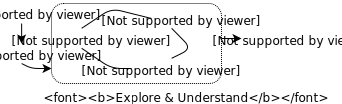
\includegraphics[width=\textwidth]{images/workflow} 

}

\caption{(ref:workflow)}\label{fig:workflow}
\end{figure}

In fact, packages within the \textbf{tidyverse} such as \textbf{dplyr} (transformation) and \textbf{ggplot2} (visualization) are such productive tools that many analysts use \emph{static} \textbf{ggplot2} graphics for EDA. Then, when it comes to communicating results, some analysts switch to another tool or language altogether (e.g., JavaScript) to generate interactive web graphics presenting their most important findings \citep{flowingdata-r, nyt-r}. Unfortunately, this requires a heavy context switch that requires a totally different skillset and impedes productivity. Moreover, for the average analyst, the opportunity costs involved with becoming competent with the complex world of web technologies is simply not worth the required investment.

Even before the web, interactive graphics were shown to have great promise in aiding the exploration of high-dimensional data \citep{Cook:2007uk}. The ASA maintains an incredible video library, \url{http://stat-graphics.org/movies/}, documenting the use of interactive statistical graphics for tasks that otherwise wouldn't have been easy or possible using numerical summaries and/or static graphics alone. Roughly speaking, these tasks tend to fall under three categories:

\begin{itemize}
\tightlist
\item
  Identifying structure that would otherwise go missing \citep{prim9}.
\item
  Diagnosing models and understanding algorithms \citep{model-vis-paper}.
\item
  Aiding the sense-making process by searching for information quickly without fully specified questions \citep{Unwin:1999vp}.
\end{itemize}

Today, you can find and run some of these and similar Graphical User Interface (GUI) systems for creating interactive graphics: \texttt{DataDesk} \url{https://datadescription.com/}, \texttt{GGobi} \url{http://www.ggobi.org/}, \texttt{Mondrian} \url{http://www.theusrus.de/Mondrian/}, \texttt{JMP} \url{https://www.jmp.com}, \texttt{Tableau} \url{https://www.tableau.com/}. Although these GUI-based systems have nice properties, they don't gel with a code-based workflow: any tasks you complete through a GUI likely can't be replicated without human intervention. That means, if at any point, the data changes, and analysis outputs must be regenerated, you need to remember precisely how to reproduce the outcome, which isn't necessarily easy, trustworthy, or economical. Moreover, GUI-based systems are typically `closed' systems that don't allow themselves to be easily customized, extended, or integrated with another system.

Programming interactive graphics allows you to leverage all the benefits of a code-based workflow while also helping with tasks that are difficult to accomplish with code alone. For an example, if you were to visualize engine displacement (\texttt{displ}) versus miles per gallon (\texttt{hwy}) using the \texttt{mpg} dataset, you might wonder: ``what are these cars with an unusually high value of \texttt{hwy} given their \texttt{displ}?''. Rather than trying to write code to query those observations, it would be more easier and intuitive to draw an outline around the points to query the data behind them.

\begin{Shaded}
\begin{Highlighting}[]
\KeywordTok{library}\NormalTok{(ggplot2)}
\KeywordTok{ggplot}\NormalTok{(mpg, }\KeywordTok{aes}\NormalTok{(displ, hwy)) }\OperatorTok{+}\StringTok{ }\KeywordTok{geom_point}\NormalTok{()}
\end{Highlighting}
\end{Shaded}

\begin{figure}

{\centering \includegraphics[width=\textwidth]{plotly_book_files/figure-latex/mpg-static-1} 

}

\caption{(ref:mpg-static)}\label{fig:mpg-static}
\end{figure}

Figure \ref{fig:mpg-lasso} demonstrates how we can transform Figure \ref{fig:mpg-static} into an interactive version that can be used to query and inspect points of interest. The framework that enables this kind of linked brushing is discussed in depth within Section \ref{graphical-queries}, but the point here is that the added effort required to enable such functionality is relatively small. This is important, because although interactivity \emph{can} augment exploration by allowing us to pursue follow-up questions, it's typically only \emph{practical} when we can create and alter them quickly. That's because, in a true exploratory setting, you have to make lots of visualizations, and investigate lots of follow-up questions, before stumbling across something truly valuable.

\begin{Shaded}
\begin{Highlighting}[]
\KeywordTok{library}\NormalTok{(plotly)}
\NormalTok{m <-}\StringTok{ }\KeywordTok{highlight_key}\NormalTok{(mpg)}
\NormalTok{p <-}\StringTok{ }\KeywordTok{ggplot}\NormalTok{(m, }\KeywordTok{aes}\NormalTok{(displ, hwy)) }\OperatorTok{+}\StringTok{ }\KeywordTok{geom_point}\NormalTok{()}
\NormalTok{gg <-}\StringTok{ }\KeywordTok{highlight}\NormalTok{(}\KeywordTok{ggplotly}\NormalTok{(p), }\StringTok{"plotly_selected"}\NormalTok{)}
\NormalTok{crosstalk}\OperatorTok{::}\KeywordTok{bscols}\NormalTok{(gg, DT}\OperatorTok{::}\KeywordTok{datatable}\NormalTok{(m))}
\end{Highlighting}
\end{Shaded}

\begin{figure}

{\centering \includegraphics[width=\textwidth]{vimeo-images/324366759/final} 

}

\caption{(ref:mpg-lasso)}\label{fig:mpg-lasso}
\end{figure}

When a valuable insight surfaces, since the code behind Figure \ref{fig:mpg-lasso} generates HTML, the web-based graphic can be easily shared with collaborators through email and/or incorporated inside a larger automated report or website. Moreover, since these interactive graphics are based on the \textbf{htmlwidgets} framework, they work seamlessly inside of larger \textbf{rmarkdown} documents, inside \textbf{shiny} apps, \texttt{RStudio}, \texttt{Jupyter} notebooks, the \texttt{R} prompt, and more. Being able to share interactive graphics with collaborators through these different mediums enhances the conversation -- your colleagues can point out things you may not yet have considered and, in some cases, they can get immediate responses from the graphics themselves.

In the final stages of an analysis, when it comes time to publish your work to a general audience, rather than relying on the audience to interact with the graphics and discover insight for themselves, it's always a good idea to clearly highlight your findings. For example, from Figure \ref{fig:mpg-lasso}, we've learned that most of these unusual points can be explained by a single feature of the data (\texttt{model\ ==\ \textquotesingle{}corvette\textquotesingle{}}). As shown in Figure \ref{fig:mpg-mark-hull}, the \texttt{geom\_mark\_hull()} function from the \textbf{ggforce} package provides a helpful way to annotate those points with a hull. Moreover, as Chapter \ref{editing-views} demonstrates, it can also be helpful to add and/or edit annotations interactively when preparing a graphic for publication.

\begin{Shaded}
\begin{Highlighting}[]
\KeywordTok{library}\NormalTok{(ggforce)}
\KeywordTok{ggplot}\NormalTok{(mpg, }\KeywordTok{aes}\NormalTok{(displ, hwy)) }\OperatorTok{+}\StringTok{ }
\StringTok{  }\KeywordTok{geom_point}\NormalTok{() }\OperatorTok{+}
\StringTok{  }\KeywordTok{geom_mark_hull}\NormalTok{(}\KeywordTok{aes}\NormalTok{(}\DataTypeTok{filter =}\NormalTok{ model }\OperatorTok{==}\StringTok{ "corvette"}\NormalTok{, }\DataTypeTok{label =}\NormalTok{ model)) }\OperatorTok{+}
\StringTok{  }\KeywordTok{labs}\NormalTok{(}
    \DataTypeTok{title =} \StringTok{"Fuel economy from 1999 to 2008 for 38 car models"}\NormalTok{,}
    \DataTypeTok{caption =} \StringTok{"Source: https://fueleconomy.gov/"}\NormalTok{,}
    \DataTypeTok{x =} \StringTok{"Engine Displacement"}\NormalTok{, }
    \DataTypeTok{y =} \StringTok{"Miles Per Gallon"}
\NormalTok{  )}
\end{Highlighting}
\end{Shaded}

\begin{figure}

{\centering \includegraphics[width=\textwidth]{plotly_book_files/figure-latex/mpg-mark-hull-1} 

}

\caption{(ref:mpg-mark-hull)}\label{fig:mpg-mark-hull}
\end{figure}

This simple example quickly shows how interactive web graphics can assist EDA (for another, slightly more in-depth example, see Section \ref{intro-ggplotly}). Being able to program these graphics from \texttt{R} allows one to combine their functionality within a world-class computing environment for data analysis and statistics. Programming interactive graphics may not be as intuitive as using a GUI-based system, but making the investment pays dividends in terms of workflow improvements: automation, scaling, provenance, and flexibility.

\hypertarget{what-you-will-learn}{%
\section{What you will learn}\label{what-you-will-learn}}

This book provides a foundation for learning how to make interactive web-based graphics for data analysis from \texttt{R} via \textbf{plotly}, without assuming any prior experience with web technologies. The goal is to provide the context you need to go beyond copying existing \textbf{plotly} examples to having a useful mental model of the underlying framework, its capabilities, and how it fits into the larger R ecosystem. By learning this mental model, you'll have a better understanding of how to create more sophisticated visualizations, fix common issues, improve performance, understand the limitations, and even contribute back to the project itself. You may already be familiar with existing \textbf{plotly} documentation (e.g., \url{https://plot.ly/r/}), which is essentially a language-agnostic how-to guide, but this book is meant to be more holistic tutorial written by and for the R user.

This book also focuses primarily on features that are unique to the \textbf{plotly} R package (i.e., things that don't work the same for Python or JavaScript). This ranges from creation of a single graph using the \texttt{plot\_ly()} special named arguments that make it easier to map data to visuals:

\begin{Shaded}
\begin{Highlighting}[]
\KeywordTok{plot_ly}\NormalTok{(diamonds, }\DataTypeTok{x =} \OperatorTok{~}\NormalTok{cut, }\DataTypeTok{color =} \OperatorTok{~}\NormalTok{clarity, }\DataTypeTok{colors =} \StringTok{"Accent"}\NormalTok{)}
\end{Highlighting}
\end{Shaded}

\begin{figure}

{\centering \includegraphics[width=\textwidth]{vimeo-images/315707813/final} 

}

\caption{(ref:intro-show-hide-preview)}\label{fig:intro-show-hide-preview}
\end{figure}

To its ability to link multiple data views purely client-side (see Section \ref{graphical-queries}):

\begin{figure}

{\centering \includegraphics[width=\textwidth]{vimeo-images/257149623/final} 

}

\caption{(ref:storms-preview)}\label{fig:storms-preview}
\end{figure}

To advanced server-side linking with \textbf{shiny} to implement responsive and scalable crossfilters (see Section \ref{crossfilter}):

\begin{figure}

{\centering \includegraphics[width=\textwidth]{vimeo-images/318129502/final} 

}

\caption{(ref:shiny-crossfilter-preview)}\label{fig:shiny-crossfilter-preview}
\end{figure}

By going through the code behind these examples, you'll see that many of them leverage other \texttt{R} packages in their implementation. To highlight a few of the R packages that you'll see:

\begin{itemize}
\tightlist
\item
  \textbf{dplyr} and \textbf{tidyr}

  \begin{itemize}
  \tightlist
  \item
    For transforming data into a form suitable for the visualization method.
  \end{itemize}
\item
  \textbf{ggplot2} and friends (e.g., \textbf{GGally}, \textbf{ggmosaic}, etc)

  \begin{itemize}
  \tightlist
  \item
    For creating \textbf{plotly} visualizations that would be tedious to implement without \texttt{ggplotly()}.
  \end{itemize}
\item
  \textbf{sf}, \textbf{rnaturalearth}, \textbf{cartogram}

  \begin{itemize}
  \tightlist
  \item
    For obtaining and working with geo-spatial data structures in R.
  \end{itemize}
\item
  \textbf{stats}, \textbf{MASS}, \textbf{broom}, and \textbf{forecast}

  \begin{itemize}
  \tightlist
  \item
    For working with statistical models and summaries.
  \end{itemize}
\item
  \textbf{shiny}

  \begin{itemize}
  \tightlist
  \item
    For running R code in response to user input.
  \end{itemize}
\item
  \textbf{htmltools}, \textbf{htmlwidgets}

  \begin{itemize}
  \tightlist
  \item
    For combining multiple views and saving the result.
  \end{itemize}
\end{itemize}

This book contains six parts and each part contains numerous chapters. A summary of each part is provided below.

\begin{enumerate}
\def\labelenumi{\arabic{enumi}.}
\item
  \emph{Creating views:} introduces the process of transforming data into graphics via \textbf{plotly}'s programmatic interface. It focuses mostly on \texttt{plot\_ly()}, which can interface directly with the underlying plotly.js graphing library, but emphasis is put on features unique to the \texttt{R} package that make it easier to transform data into graphics. Another way to create graphs with \textbf{plotly} is to use the \texttt{ggplotly()} function to transform \textbf{ggplot2} graphs into \textbf{plotly} graphs. Section \ref{intro-ggplotly} discusses when and why \texttt{ggplotly()} might be desirable to \texttt{plot\_ly()}. It's also worth mentioning that this part (nor the book as a whole) does not intend to cover every possible chart type and option available in \textbf{plotly} -- it's more of a presentation of the most generally useful techniques with the greater \texttt{R} ecosystem in mind. For a more exhaustive gallery of examples of what \textbf{plotly} itself is capable of, see \url{https://plot.ly/r/}.
\item
  \emph{Publishing views:} discusses various techniques for exporting (as well as embedding) \textbf{plotly} graphs to various file formats (e.g., HTML, svg, pdf, png, etc). Also, Chapter \ref{editing-views} demonstrates how one could leverage editable layout components HTML to touch-up a graph, then export to a static file format of interest before publication. Indeed, this book was created using the techniques from this section.
\item
  \emph{Combining multiple views:} demonstrates how to combine multiple data views into a single web page (arranging) or graphic (animation). Most of these techniques are shown using \textbf{plotly} graphs, but techniques from Section \ref{arranging-htmlwidgets} extend to any HTML content generated via \textbf{htmltools} (which includes \textbf{htmlwidgets}).
\item
  \emph{Linking multiple views:} provides an overview of the two models for linking \textbf{plotly} graph(s) to other data views. The first model, covered in Section \ref{graphical-queries}, outlines \textbf{plotly}'s support for linking views purely client-side, meaning the resulting graphs render in any web browser on any machine without requiring external software. The second model, covered in Chapter \ref{linking-views-with-shiny}, demonstrates how to link \textbf{plotly} with other views via \textbf{shiny}, a reactive web application framework for \texttt{R}. Relatively speaking, the second model grants the \texttt{R} user way more power and flexibility, but comes at the cost of requiring more computational infrastructure. That being said, RStudio provides accessible resources for deploying \textbf{shiny} apps \url{https://shiny.rstudio.com/articles/\#deployment}.
\item
  \emph{Custom behavior with JavaScript:} demonstrates various ways to customize \textbf{plotly} graphs by writing custom JavaScript to handle certain user events. This part of the book is designed to be approachable for \texttt{R} users that want to learn just enough JavaScript to \textbf{plotly} to do something it doesn't ``natively'' support.
\item
  \emph{Various special topics}: offers a grab-bag of topics that address common questions, mostly related to the customization of \textbf{plotly} graphs in \texttt{R}.
\end{enumerate}

You might already notice that this book often uses the term `view' or `data view', so here we take a moment to frame its use in a wider context. As \citet{Wills2008} puts it: ``a `data view' is anything that gives the user a way of examining data so as to gain insight and understanding. A data view is usually thought of as a barchart, scatterplot, or other traditional statistical graphic, but we use the term more generally, including `views' such as the results of a regression analysis, a neural net prediction, or a set of descriptive statistics''. In this book, more often than not, the term `view' typically refers to a \textbf{plotly} graph or other \textbf{htmlwidgets} (e.g., \textbf{DT}, \textbf{leaflet}, etc). In particular, Section \ref{graphical-queries} is all about linking multiple \textbf{htmlwidgets} together through a graphical database querying framework. However, the term `view' takes on a more general interpretation in Chapter \ref{linking-views-with-shiny} since the reactive programming framework that \textbf{shiny} provides allows us to have a more general conversation surrounding linked data views.

\hypertarget{what-you-wont-learn-much-of}{%
\section{What you won't learn (much of)}\label{what-you-wont-learn-much-of}}

\hypertarget{web-technologies}{%
\subsection{Web technologies}\label{web-technologies}}

Although this book is fundamentally about creating web graphics, it does not aim to teach you web technologies (e.g., HTML, SVG, CSS, JavaScript, etc). It's true that mastering these technologies grants you the ability to build really impressive websites, but even expert web developers would say their skillset is much better suited for expository rather than exploratory visualization. That's because, most web programming tools are not well-suited for the exploratory phase of a data science workflow where iteration between data visualization, transformation, and modeling is a necessary task that often impedes hypothesis generation and sense-making. As a result, for most data analysts whose primary function is to derive insight from data, the opportunity costs involved with mastering web technologies is usually not worth the investment.

That being said, learning a little about web technologies can have a relatively large payoff with directed learning and instruction. In Chapter \ref{javascript}, you'll learn how to customize \textbf{plotly} graphs with JavaScript -- even if you haven't seen JavaScript before, this chapter should be approachable, insightful, and provide you with some useful examples.

\hypertarget{d3js}{%
\subsection{d3js}\label{d3js}}

The JavaScript library D3 is a great tool for data visualization assuming you're familiar with web technologies and are primarily interested in expository (not exploratory) visualization. There are already lots of great resources for learning D3, including the numerous books by \citet{murray-d3} and \citet{meeks-d3}. It's worth noting, however, if you do know D3, you can easily leverage it from a web page that are already a \textbf{plotly} graph, as demonstrated in Figure \ref{fig:correlation-client-side}.

\hypertarget{ggplot2}{%
\subsection{ggplot2}\label{ggplot2}}

The book does contain some \textbf{ggplot2} code examples (which are then converted to \textbf{plotly} via \texttt{ggplotly()}), but it's not designed to teach you \textbf{ggplot2}. For those looking to learn \textbf{ggplot2}, I recommend using the learning materials listed at \url{https://ggplot2.tidyverse.org}.

\hypertarget{graphical-data-analysis}{%
\subsection{Graphical data analysis}\label{graphical-data-analysis}}

How to perform data analysis via graphics (carefully, correctly, and creatively) is a large topic unto itself. Although this book does have examples of graphical data analysis, it does not aim to provide a comprehensive foundation. For nice comprehensive resources on the topic, see \citet{unwin-graphical-analysis} and \citet{ggobi:2007}.

\hypertarget{data-visualization-best-practices}{%
\subsection{Data visualization best practices}\label{data-visualization-best-practices}}

Encoding information in a graphic (concisely and effectively) is a large topic unto itself. Although this book does have some ramblings related to best practices in data visualization, it does not aim to provide a comprehensive foundation. For some approachable and fun resources on the topic, see \citet{tufte-dataviz}, \citet{yau-dataviz}, \citet{healey-dataviz}, and \citet{claus-dataviz}.

\hypertarget{prerequisites}{%
\section{Prerequisites}\label{prerequisites}}

For those new to \texttt{R} and/or data visualization, \href{https://r4ds.had.co.nz/}{R for Data Science} provides an excellent foundation for understanding the vast majority of concepts covered in this book \citep{r4ds}. In particular, if you have a solid grasp on \href{https://r4ds.had.co.nz/explore-intro.html}{Part I: Explore}, \href{https://r4ds.had.co.nz/wrangle-intro.html}{Part II: Wrangle}, and \href{https://r4ds.had.co.nz/program-intro.html}{Part III: Program}, you should be able to understand almost everything here. Although not explicitly covered, the book does make references to (and was creating using) \textbf{rmarkdown}, so if you're new to \textbf{rmarkdown}, I also recommend reading the \href{https://r4ds.had.co.nz/r-markdown.html}{R Markdown chapter}.

\hypertarget{run-code-examples}{%
\section{Run code examples}\label{run-code-examples}}

This book contains many code examples in an effort to teach the art and science behind creating interactive web-based graphics using \textbf{plotly}. To see the actual interactive result of the code (rather than a video or static version), you may want to run the code examples in a suitable computational environment. Visit \url{http://bit.ly/plotly-book-cloud} for a cloud-based instance of RStudio with all the required software to run the code examples in this book. Most, if not all of these code examples assume you have the \textbf{plotly} package loaded:

\begin{Shaded}
\begin{Highlighting}[]
\KeywordTok{library}\NormalTok{(plotly)}
\end{Highlighting}
\end{Shaded}

Within some chapters, there may be examples that assume packages we loaded during a previous example. If you'd like to avoid this situation, please load the

\begin{Shaded}
\begin{Highlighting}[]
\KeywordTok{library}\NormalTok{(plotlyBook)}
\end{Highlighting}
\end{Shaded}

If you'd like to run examples on your local machine (instead of RStudio Cloud), you can install all the necessary R packages with:

\begin{Shaded}
\begin{Highlighting}[]
\ControlFlowTok{if}\NormalTok{ (}\OperatorTok{!}\KeywordTok{require}\NormalTok{(remotes)) }\KeywordTok{install.packages}\NormalTok{(}\StringTok{"remotes"}\NormalTok{)}
\NormalTok{remotes}\OperatorTok{::}\KeywordTok{install_github}\NormalTok{(}\StringTok{"cpsievert/plotly_book"}\NormalTok{)}
\end{Highlighting}
\end{Shaded}

\hypertarget{getting-help-and-learning-more}{%
\section{Getting help and learning more}\label{getting-help-and-learning-more}}

As \citet{r4ds} states, ``This book is not an island; there is no single resource that will allow you to master \texttt{R} {[}or \textbf{plotly}{]}. As you start to apply the techniques described in this book to your own data you will soon find questions that I do not answer. This section describes a few tips on how to get help, and to help you keep learning.'' \href{https://r4ds.had.co.nz/introduction.html\#getting-help-and-learning-more}{These tips} on how to get help (e.g., Google, StackOverflow, Twitter, etc) also apply to getting help with \textbf{plotly}. \href{https://community.rstudio.com/tags/plotly}{RStudio's community} is another great place to ask broader questions about all things \texttt{R} and \textbf{plotly}. It's worth mentioning that the \texttt{R} community is incredibly welcoming, compassionate, and generous; especially if you can demonstrate that you've done your research and/or \href{https://www.tidyverse.org/help/}{provide minimally reproducible example of your problem}.

\hypertarget{acknowledgements}{%
\section{Acknowledgements}\label{acknowledgements}}

This book wouldn't be possible without the generous assistance and mentorship of many people:

\begin{itemize}
\tightlist
\item
  Heike Hofmann and Di Cook for their mentorship and many helpful conversations about interactive graphics.
\item
  Toby Dylan Hocking for many helpful conversations, his mentorship in the \texttt{R} packages \textbf{animint} and \textbf{plotly}, and laying the original foundation behind \texttt{ggplotly()}.
\item
  Joe Cheng for many helpful conversations and inspiring Section \ref{graphical-queries}.
\item
  Étienne Tétreault-Pinard, Alex Johnson, and the other plotly.js core developers for responding to my feature requests and bug reports.
\item
  Yihui Xie for his work on \textbf{knitr}, \textbf{rmarkdown}, \textbf{bookdown}, \href{https://github.com/yihui/bookdown-crc}{bookdown-crc}, and responding to my feature requests.
\item
  Anthony Unwin for helpful feedback, suggestions, and for inspiring Figure \ref{fig:epl}.
\item
  Hadley Wickham and the \textbf{ggplot2} team for maintaining \textbf{ggplot2}.
\item
  Hadley Wickham and Garret Grolemund for writing \emph{R for Data Science} and allowing me to model this introduction after their introduction.
\item
  Kent Russell for contributions to \textbf{plotly} and writing \textbf{reactR}.
\item
  Adam Loy for inspiring Figure \ref{fig:profile-pyramid}.
\item
  Many other R community members who contributed to the \textbf{plotly} package and provided feedback and corrections for this book.
\end{itemize}

\hypertarget{colophon}{%
\section{Colophon}\label{colophon}}

An online version of this book is available at \url{https://plotly-r.com}. It will continue to evolve in between reprints of the physical book. The source of the book is available at \url{https://github.com/cpsievert/plotly_book}. The book is powered by \url{https://bookdown.org} which makes it easy to turn \texttt{R} markdown files into HTML, PDF, and EPUB.

This book was built with the following computing environment:

\begin{Shaded}
\begin{Highlighting}[]
\NormalTok{devtools}\OperatorTok{::}\KeywordTok{session_info}\NormalTok{(}\StringTok{"plotly"}\NormalTok{)}
\CommentTok{#> - Session info --------------------------------------}
\CommentTok{#>  setting  value                       }
\CommentTok{#>  version  R version 3.6.1 (2019-07-05)}
\CommentTok{#>  os       macOS Mojave 10.14.5        }
\CommentTok{#>  system   x86_64, darwin15.6.0        }
\CommentTok{#>  ui       X11                         }
\CommentTok{#>  language (EN)                        }
\CommentTok{#>  collate  en_US.UTF-8                 }
\CommentTok{#>  ctype    en_US.UTF-8                 }
\CommentTok{#>  tz       America/Chicago             }
\CommentTok{#>  date     2019-10-01                  }
\CommentTok{#> }
\CommentTok{#> - Packages ------------------------------------------}
\CommentTok{#>  package      * version    date       lib}
\CommentTok{#>  askpass        1.1        2019-01-13 [1]}
\CommentTok{#>  assertthat     0.2.1      2019-03-21 [1]}
\CommentTok{#>  backports      1.1.4      2019-04-10 [1]}
\CommentTok{#>  base64enc      0.1-3      2015-07-28 [1]}
\CommentTok{#>  BH             1.69.0-1   2019-01-07 [1]}
\CommentTok{#>  cli            1.1.0      2019-03-19 [1]}
\CommentTok{#>  colorspace     1.4-1      2019-03-18 [1]}
\CommentTok{#>  crayon         1.3.4      2017-09-16 [1]}
\CommentTok{#>  crosstalk      1.0.0      2016-12-21 [1]}
\CommentTok{#>  curl           4.2        2019-09-24 [1]}
\CommentTok{#>  data.table     1.12.2     2019-04-07 [1]}
\CommentTok{#>  digest         0.6.21     2019-09-20 [1]}
\CommentTok{#>  dplyr          0.8.3      2019-07-04 [1]}
\CommentTok{#>  ellipsis       0.3.0      2019-09-20 [1]}
\CommentTok{#>  fansi          0.4.0      2018-10-05 [1]}
\CommentTok{#>  fastmap        1.0.0      2019-08-02 [1]}
\CommentTok{#>  ggplot2      * 3.2.1.9000 2019-10-01 [1]}
\CommentTok{#>  glue           1.3.1      2019-03-12 [1]}
\CommentTok{#>  gtable         0.3.0      2019-03-25 [1]}
\CommentTok{#>  hexbin         1.27.3     2019-05-14 [1]}
\CommentTok{#>  htmltools      0.4.0      2019-09-17 [1]}
\CommentTok{#>  htmlwidgets    1.5        2019-09-26 [1]}
\CommentTok{#>  httpuv         1.5.2      2019-09-11 [1]}
\CommentTok{#>  httr           1.4.1      2019-08-05 [1]}
\CommentTok{#>  jsonlite       1.6        2018-12-07 [1]}
\CommentTok{#>  labeling       0.3        2014-08-23 [1]}
\CommentTok{#>  later          1.0.0      2019-09-17 [1]}
\CommentTok{#>  lattice        0.20-38    2018-11-04 [1]}
\CommentTok{#>  lazyeval       0.2.2      2019-03-15 [1]}
\CommentTok{#>  lifecycle      0.1.0      2019-08-01 [1]}
\CommentTok{#>  magrittr       1.5        2014-11-22 [1]}
\CommentTok{#>  MASS           7.3-51.4   2019-03-31 [1]}
\CommentTok{#>  Matrix         1.2-17     2019-03-22 [1]}
\CommentTok{#>  mgcv           1.8-29     2019-09-20 [1]}
\CommentTok{#>  mime           0.7        2019-06-11 [1]}
\CommentTok{#>  munsell        0.5.0      2018-06-12 [1]}
\CommentTok{#>  nlme           3.1-141    2019-08-01 [1]}
\CommentTok{#>  openssl        1.4.1      2019-07-18 [1]}
\CommentTok{#>  pillar         1.4.2      2019-06-29 [1]}
\CommentTok{#>  pkgconfig      2.0.3      2019-09-22 [1]}
\CommentTok{#>  plogr          0.2.0      2018-03-25 [1]}
\CommentTok{#>  plotly         4.9.0.9000 2019-09-23 [1]}
\CommentTok{#>  plyr           1.8.4      2016-06-08 [1]}
\CommentTok{#>  promises       1.1.0      2019-09-25 [1]}
\CommentTok{#>  purrr          0.3.2.9000 2019-09-30 [1]}
\CommentTok{#>  R6             2.4.0      2019-02-14 [1]}
\CommentTok{#>  RColorBrewer   1.1-2      2014-12-07 [1]}
\CommentTok{#>  Rcpp           1.0.2      2019-07-25 [1]}
\CommentTok{#>  reshape2       1.4.3      2017-12-11 [1]}
\CommentTok{#>  rlang          0.4.0.9002 2019-09-25 [1]}
\CommentTok{#>  scales         1.0.0.9000 2019-07-19 [1]}
\CommentTok{#>  shiny          1.4.0      2019-09-26 [1]}
\CommentTok{#>  sourcetools    0.1.7      2018-04-25 [1]}
\CommentTok{#>  stringi        1.4.3      2019-03-12 [1]}
\CommentTok{#>  stringr        1.4.0      2019-02-10 [1]}
\CommentTok{#>  sys            3.3        2019-08-21 [1]}
\CommentTok{#>  tibble         2.1.3      2019-06-06 [1]}
\CommentTok{#>  tidyr          1.0.0      2019-09-11 [1]}
\CommentTok{#>  tidyselect     0.2.5      2018-10-11 [1]}
\CommentTok{#>  utf8           1.1.4      2018-05-24 [1]}
\CommentTok{#>  vctrs          0.2.0.9003 2019-09-30 [1]}
\CommentTok{#>  viridisLite    0.3.0      2018-02-01 [1]}
\CommentTok{#>  withr          2.1.2      2018-03-15 [1]}
\CommentTok{#>  xtable         1.8-4      2019-04-21 [1]}
\CommentTok{#>  yaml           2.2.0      2018-07-25 [1]}
\CommentTok{#>  zeallot        0.1.0      2018-01-28 [1]}
\CommentTok{#>  source                               }
\CommentTok{#>  CRAN (R 3.6.0)                       }
\CommentTok{#>  CRAN (R 3.6.0)                       }
\CommentTok{#>  CRAN (R 3.6.0)                       }
\CommentTok{#>  CRAN (R 3.6.0)                       }
\CommentTok{#>  CRAN (R 3.6.0)                       }
\CommentTok{#>  CRAN (R 3.6.0)                       }
\CommentTok{#>  CRAN (R 3.6.0)                       }
\CommentTok{#>  CRAN (R 3.6.0)                       }
\CommentTok{#>  CRAN (R 3.6.0)                       }
\CommentTok{#>  CRAN (R 3.6.1)                       }
\CommentTok{#>  CRAN (R 3.6.0)                       }
\CommentTok{#>  CRAN (R 3.6.1)                       }
\CommentTok{#>  CRAN (R 3.6.0)                       }
\CommentTok{#>  CRAN (R 3.6.1)                       }
\CommentTok{#>  CRAN (R 3.6.0)                       }
\CommentTok{#>  Github (r-lib/fastmap@b104c2c)       }
\CommentTok{#>  local                                }
\CommentTok{#>  CRAN (R 3.6.0)                       }
\CommentTok{#>  CRAN (R 3.6.0)                       }
\CommentTok{#>  CRAN (R 3.6.0)                       }
\CommentTok{#>  Github (rstudio/htmltools@0366ff7)   }
\CommentTok{#>  Github (ramnathv/htmlwidgets@7bcb531)}
\CommentTok{#>  CRAN (R 3.6.1)                       }
\CommentTok{#>  CRAN (R 3.6.1)                       }
\CommentTok{#>  CRAN (R 3.6.0)                       }
\CommentTok{#>  CRAN (R 3.6.0)                       }
\CommentTok{#>  Github (r-lib/later@0364de9)         }
\CommentTok{#>  CRAN (R 3.6.1)                       }
\CommentTok{#>  CRAN (R 3.6.0)                       }
\CommentTok{#>  CRAN (R 3.6.0)                       }
\CommentTok{#>  CRAN (R 3.6.0)                       }
\CommentTok{#>  CRAN (R 3.6.1)                       }
\CommentTok{#>  CRAN (R 3.6.1)                       }
\CommentTok{#>  CRAN (R 3.6.0)                       }
\CommentTok{#>  CRAN (R 3.6.0)                       }
\CommentTok{#>  CRAN (R 3.6.0)                       }
\CommentTok{#>  CRAN (R 3.6.0)                       }
\CommentTok{#>  CRAN (R 3.6.1)                       }
\CommentTok{#>  CRAN (R 3.6.0)                       }
\CommentTok{#>  CRAN (R 3.6.1)                       }
\CommentTok{#>  CRAN (R 3.6.0)                       }
\CommentTok{#>  local                                }
\CommentTok{#>  CRAN (R 3.6.0)                       }
\CommentTok{#>  Github (rstudio/promises@39faf86)    }
\CommentTok{#>  Github (tidyverse/purrr@9edf0ca)     }
\CommentTok{#>  CRAN (R 3.6.0)                       }
\CommentTok{#>  CRAN (R 3.6.0)                       }
\CommentTok{#>  CRAN (R 3.6.1)                       }
\CommentTok{#>  CRAN (R 3.6.0)                       }
\CommentTok{#>  Github (r-lib/rlang@03bc5ed)         }
\CommentTok{#>  Github (r-lib/scales@7f6f4a5)        }
\CommentTok{#>  Github (rstudio/shiny@ff3f7ad)       }
\CommentTok{#>  CRAN (R 3.6.0)                       }
\CommentTok{#>  CRAN (R 3.6.0)                       }
\CommentTok{#>  CRAN (R 3.6.0)                       }
\CommentTok{#>  CRAN (R 3.6.0)                       }
\CommentTok{#>  CRAN (R 3.6.0)                       }
\CommentTok{#>  CRAN (R 3.6.0)                       }
\CommentTok{#>  CRAN (R 3.6.0)                       }
\CommentTok{#>  CRAN (R 3.6.0)                       }
\CommentTok{#>  Github (r-lib/vctrs@7ab6f81)         }
\CommentTok{#>  CRAN (R 3.6.0)                       }
\CommentTok{#>  CRAN (R 3.6.0)                       }
\CommentTok{#>  CRAN (R 3.6.0)                       }
\CommentTok{#>  CRAN (R 3.6.0)                       }
\CommentTok{#>  CRAN (R 3.6.0)                       }
\CommentTok{#> }
\CommentTok{#> [1] /Library/Frameworks/R.framework/Versions/3.6/Resources/library}
\end{Highlighting}
\end{Shaded}

\hypertarget{scatter-traces}{%
\chapter{Scattered foundations}\label{scatter-traces}}

As we learned in Section \ref{intro-plotly-js}, a plotly.js figure contains one (or more) trace(s), and every trace has a type. The trace type scatter is great for drawing low-level geometries (e.g., points, lines, text, and polygons) and provides the foundation for many \texttt{add\_*()} functions (e.g., \texttt{add\_markers()}, \texttt{add\_lines()}, \texttt{add\_paths()}, \texttt{add\_segments()}, \texttt{add\_ribbons()}, \texttt{add\_area()}, and \texttt{add\_polygons()}) as well as many \texttt{ggplotly()} charts. These scatter-based layers provide a more convenient interface to special cases of the scatter trace by doing a bit of data wrangling and transformation under-the-hood before mapping to scatter trace(s). For a simple example, \texttt{add\_lines()} ensures lines are drawn according to the ordering of \texttt{x}, which is desirable for a time series plotting. This behavior is subtly different than \texttt{add\_paths()} which uses row ordering instead.

\begin{Shaded}
\begin{Highlighting}[]
\KeywordTok{library}\NormalTok{(plotly)}
\KeywordTok{data}\NormalTok{(economics, }\DataTypeTok{package =} \StringTok{"ggplot2"}\NormalTok{)}

\CommentTok{# sort economics by psavert, just to }
\CommentTok{# show difference between paths and lines}
\NormalTok{p <-}\StringTok{ }\NormalTok{economics }\OperatorTok
\StringTok{  }\KeywordTok{arrange}\NormalTok{(psavert) }\OperatorTok
\StringTok{  }\KeywordTok{plot_ly}\NormalTok{(}\DataTypeTok{x =} \OperatorTok{~}\NormalTok{date, }\DataTypeTok{y =} \OperatorTok{~}\NormalTok{psavert)}

\KeywordTok{add_paths}\NormalTok{(p)}
\KeywordTok{add_lines}\NormalTok{(p)}
\end{Highlighting}
\end{Shaded}

\begin{figure}

{\centering \includegraphics[width=\textwidth]{images/scatter-intro} 

}

\caption{(ref:scatter-intro)}\label{fig:scatter-intro}
\end{figure}

Section \ref{intro-plotly} introduced `aesthetic mapping' arguments (unique to the R package) which make it easier to map data to visual properties (e.g., \texttt{color}, \texttt{linetype}, etc). In addition to these arguments, \textbf{dplyr} groupings can be used to ensure there is at least one geometry per group. The top panel of Figure \ref{fig:scatter-intro} demonstrates how \texttt{group\_by()} could be used to effectively wrap the time series from Figure \ref{fig:scatter-intro} by year, which can be useful for visualizing annual seasonality. Another approach to generating at least one geometry per `group' is to provide categorical variable to a relevant aesthetic (e.g., \texttt{color}), as shown in the bottom panel of Figure \ref{fig:scatter-intro}.

\begin{Shaded}
\begin{Highlighting}[]
\KeywordTok{library}\NormalTok{(lubridate)}
\NormalTok{econ <-}\StringTok{ }\NormalTok{economics }\OperatorTok
\StringTok{  }\KeywordTok{mutate}\NormalTok{(}\DataTypeTok{yr =} \KeywordTok{year}\NormalTok{(date), }\DataTypeTok{mnth =} \KeywordTok{month}\NormalTok{(date))}

\CommentTok{# One trace (more performant, but less interactive)}
\NormalTok{econ }\OperatorTok
\StringTok{  }\KeywordTok{group_by}\NormalTok{(yr) }\OperatorTok
\StringTok{  }\KeywordTok{plot_ly}\NormalTok{(}\DataTypeTok{x =} \OperatorTok{~}\NormalTok{mnth, }\DataTypeTok{y =} \OperatorTok{~}\NormalTok{uempmed) }\OperatorTok
\StringTok{  }\KeywordTok{add_lines}\NormalTok{(}\DataTypeTok{text =} \OperatorTok{~}\NormalTok{yr)}

\CommentTok{# Multiple traces (less performant, but more interactive)}
\KeywordTok{plot_ly}\NormalTok{(econ, }\DataTypeTok{x =} \OperatorTok{~}\NormalTok{mnth, }\DataTypeTok{y =} \OperatorTok{~}\NormalTok{uempmed) }\OperatorTok
\StringTok{  }\KeywordTok{add_lines}\NormalTok{(}\DataTypeTok{color =} \OperatorTok{~}\KeywordTok{ordered}\NormalTok{(yr))}
  
\CommentTok{# The split argument guarantees one trace per group level (regardless }
\CommentTok{# of the variable type). This is useful if you want a consistent visual}
\CommentTok{# property over multiple traces }
\CommentTok{# plot_ly(econ, x = ~mnth, y = ~uempmed) %>%}
\CommentTok{#   add_lines(split = ~yr, color = I("black"))}
\end{Highlighting}
\end{Shaded}

\begin{figure}

{\centering \includegraphics[width=\textwidth]{vimeo-images/316679591/final} 

}

\caption{(ref:scatter-lines)}\label{fig:scatter-lines}
\end{figure}

Not only do these plots differ in visual appearance, they also differ in interactive capabilities, computational performance, and underlying implementation. That's because, the grouping approach (top panel of Figure \ref{fig:scatter-lines}) uses just one plotly.js trace (more performant, less interactive), whereas the \texttt{color} approach (bottom panel of Figure \ref{fig:scatter-lines}) generates one trace per line/year. In this case, the benefit of having multiple traces is that we can perform interactive filtering via the legend and compare multiple y-values at a given x. The cost of having those capabilities is that plots starts to be become sluggish after a few hundred traces, whereas thousands of lines can be rendered fairly easily in one trace. See Chapter \ref{performance} for more details on scaling and performance.

These features make it easier to get started using plotly.js, but it still pays off to learn how to use plotly.js directly. You won't find plotly.js attributes listed as explicit arguments in any \textbf{plotly} function (except for the special \texttt{type} attribute), but they are passed along verbatim to the plotly.js figure definition through the \texttt{...} operator. The scatter-based layers in this chapter fix the \texttt{type} plotly.js attribute to \texttt{"scatter"} as well as the \href{https://plot.ly/r/reference/\#scatter-mode}{\texttt{mode}} (e.g., \texttt{add\_markers()} uses \texttt{mode=\textquotesingle{}markers\textquotesingle{}} etc), but you could also use the lower-level \texttt{add\_trace()} to work more directly with plotly.js. For example, Figure \ref{fig:tooltip-praise} shows how to render markers, lines, and text in the same scatter trace. It also demonstrates how to leverage \emph{nested} plotly.js attributes, like \href{https://plot.ly/r/reference/\#scatter-textfont}{\texttt{textfont}} and \href{https://plot.ly/r/reference/\#layout-xaxis}{\texttt{xaxis}} -- these attributes contain other attributes, so you need to supply a suitable named list to these arguments.

\begin{Shaded}
\begin{Highlighting}[]
\KeywordTok{set.seed}\NormalTok{(}\DecValTok{99}\NormalTok{)}
\KeywordTok{plot_ly}\NormalTok{() }\OperatorTok
\StringTok{ }\KeywordTok{add_trace}\NormalTok{(}
   \DataTypeTok{type =} \StringTok{"scatter"}\NormalTok{,}
   \DataTypeTok{mode =} \StringTok{"markers+lines+text"}\NormalTok{,}
   \DataTypeTok{x =} \DecValTok{4}\OperatorTok{:}\DecValTok{6}\NormalTok{, }
   \DataTypeTok{y =} \DecValTok{4}\OperatorTok{:}\DecValTok{6}\NormalTok{,}
   \DataTypeTok{text =} \KeywordTok{replicate}\NormalTok{(}\DecValTok{3}\NormalTok{, praise}\OperatorTok{::}\KeywordTok{praise}\NormalTok{(}\StringTok{"You are $\{adjective\}! 🙌"}\NormalTok{)),}
   \DataTypeTok{textposition =} \StringTok{"right"}\NormalTok{,}
   \DataTypeTok{hoverinfo =} \StringTok{"text"}\NormalTok{,}
   \DataTypeTok{textfont =} \KeywordTok{list}\NormalTok{(}\DataTypeTok{family =} \StringTok{"Roboto Condensed"}\NormalTok{, }\DataTypeTok{size =} \DecValTok{16}\NormalTok{)}
\NormalTok{ ) }\OperatorTok
\StringTok{ }\KeywordTok{layout}\NormalTok{(}\DataTypeTok{xaxis =} \KeywordTok{list}\NormalTok{(}\DataTypeTok{range =} \KeywordTok{c}\NormalTok{(}\DecValTok{3}\NormalTok{, }\DecValTok{8}\NormalTok{)))}
\end{Highlighting}
\end{Shaded}

\begin{figure}

{\centering \includegraphics[width=\textwidth]{images/tooltip-praise} 

}

\caption{(ref:tooltip-praise)}\label{fig:tooltip-praise}
\end{figure}

If you are new to plotly.js, I recommend taking a bit of time to look through the plotly.js attributes that are available to the scatter trace type and think how you might be able to use them. Most of these attributes work for other trace types as well, so learning an attribute once for a specific plot can pay off in other contexts as well. The online plotly.js figure reference, \url{https://plot.ly/r/reference/\#scatter}, is a decent place to search and learn about the attributes, but I recommend using the \texttt{schema()} function instead for a few reasons:

\begin{itemize}
\tightlist
\item
  \texttt{schema()} provides a bit more information than the online docs (e.g., value types, default values, acceptable ranges, etc).
\item
  The interface makes it a bit easier to traverse and discover new attributes.
\item
  You can be absolutely sure it matches the version used in the R package (the online docs might use a different -- probably older -- version).
\end{itemize}

\begin{Shaded}
\begin{Highlighting}[]
\KeywordTok{schema}\NormalTok{()}
\end{Highlighting}
\end{Shaded}

\begin{figure}

{\centering \includegraphics[width=0.4\linewidth]{images/schema} 

}

\caption{(ref:schema)}\label{fig:schema}
\end{figure}

The sections that follow in this chapter demonstrate various type of data views using scatter-based layers. In attempt to avoid duplication of documentation, a particular emphasis is put on features only currently availbale from the R package (e.g., the aesthetic mapping arguments).

\hypertarget{markers}{%
\section{Markers}\label{markers}}

This section details scatter traces with a \texttt{mode} of \texttt{"markers"} (i.e., \texttt{add\_markers()}). For simplicity, many of the examples here use \texttt{add\_markers()} with a numeric x and y axis, which results in scatterplot -- a common way to visualize the association between two quantitative variables. The content that follows is still relevant markers displayed non-numeric x and y (aka dot pots) as shown in Section \ref{dot-plots}.

\hypertarget{marker-alpha}{%
\subsection{Alpha blending}\label{marker-alpha}}

As \citet{unwin-graphical-analysis} notes, scatterplots can be useful for exposing other important features including: casual relationships, outliers, clusters, gaps, barriers, and conditional relationships. A common problem with scatterplots, however is overplotting, meaning that there are multiple observations occupying the same (or similar) x/y locations. Figure \ref{fig:scatterplots} demonstrates one way to combat overplotting via alpha blending. When dealing with tens of thousands of points (or more), consider using \texttt{toWebGL()} to render plots using Canvas rather than SVG (more in Chapter \ref{performance}, or leveraging 2D density estimation (Section \ref{rectangular-binning-in-r}).

\begin{Shaded}
\begin{Highlighting}[]
\KeywordTok{subplot}\NormalTok{(}
  \KeywordTok{plot_ly}\NormalTok{(mpg, }\DataTypeTok{x =} \OperatorTok{~}\NormalTok{cty, }\DataTypeTok{y =} \OperatorTok{~}\NormalTok{hwy, }\DataTypeTok{name =} \StringTok{"default"}\NormalTok{),}
  \KeywordTok{plot_ly}\NormalTok{(mpg, }\DataTypeTok{x =} \OperatorTok{~}\NormalTok{cty, }\DataTypeTok{y =} \OperatorTok{~}\NormalTok{hwy) }\OperatorTok\StringTok{ }
\StringTok{    }\KeywordTok{add_markers}\NormalTok{(}\DataTypeTok{alpha =} \FloatTok{0.2}\NormalTok{, }\DataTypeTok{name =} \StringTok{"alpha"}\NormalTok{)}
\NormalTok{)}
\end{Highlighting}
\end{Shaded}

\begin{figure}

{\centering 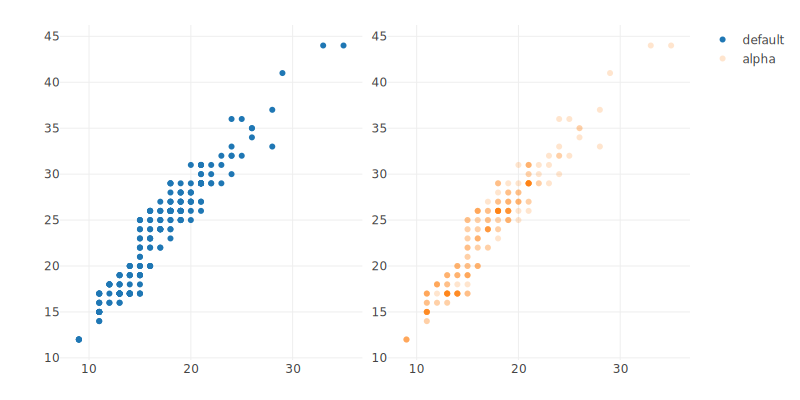
\includegraphics[width=\textwidth]{images/scatterplots} 

}

\caption{(ref:scatterplots)}\label{fig:scatterplots}
\end{figure}

\hypertarget{marker-color}{%
\subsection{Colors}\label{marker-color}}

As discussed in Section \ref{intro-plotly-js}, mapping a discrete variable to \texttt{color} produces one trace per category, which is desirable for it's legend and hover properties. On the other hand, mapping a \emph{numeric} variable to \texttt{color} produces one trace, as well as a \href{https://plot.ly/r/reference/\#scatter-marker-colorbar}{colorbar} guide for visually decoding colors back to data values. The \texttt{colorbar()} function can be used to customize the appearance of this automatically generated guide. The default colorscale is viridis, a perceptually-uniform colorscale (even when converted to black-and-white), and perceivable even to those with common forms of color blindness \citep{viridis}. Viridis is also the default colorscale for ordered factors.

\begin{Shaded}
\begin{Highlighting}[]
\NormalTok{p <-}\StringTok{ }\KeywordTok{plot_ly}\NormalTok{(mpg, }\DataTypeTok{x =} \OperatorTok{~}\NormalTok{cty, }\DataTypeTok{y =} \OperatorTok{~}\NormalTok{hwy, }\DataTypeTok{alpha =} \FloatTok{0.5}\NormalTok{)}
\KeywordTok{subplot}\NormalTok{(}
  \KeywordTok{add_markers}\NormalTok{(p, }\DataTypeTok{color =} \OperatorTok{~}\NormalTok{cyl, }\DataTypeTok{showlegend =} \OtherTok{FALSE}\NormalTok{) }\OperatorTok\StringTok{ }
\StringTok{    }\KeywordTok{colorbar}\NormalTok{(}\DataTypeTok{title =} \StringTok{"Viridis"}\NormalTok{),}
  \KeywordTok{add_markers}\NormalTok{(p, }\DataTypeTok{color =} \OperatorTok{~}\KeywordTok{factor}\NormalTok{(cyl))}
\NormalTok{)}
\end{Highlighting}
\end{Shaded}

\begin{figure}

{\centering 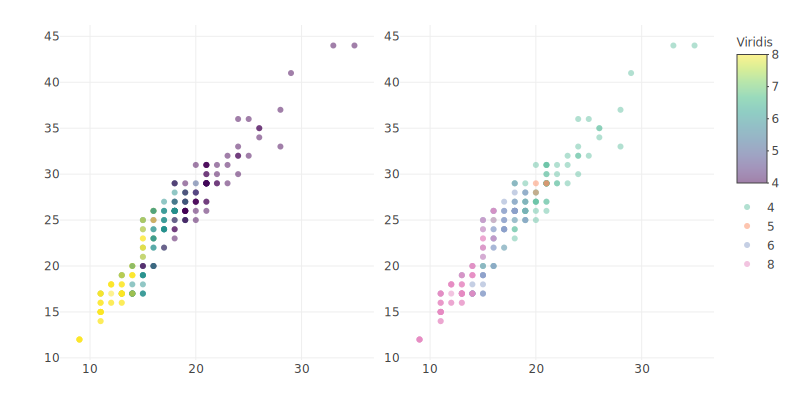
\includegraphics[width=\textwidth]{images/color-types} 

}

\caption{(ref:color-types)}\label{fig:color-types}
\end{figure}

There are numerous ways to alter the default color scale via the \texttt{colors} argument. This argument excepts one of the following: (1) a color brewer palette name (see the row names of \texttt{RColorBrewer::brewer.pal.info} for valid names), (2) a vector of colors to interpolate, or (3) a color interpolation function like \texttt{colorRamp()} or \texttt{scales::colour\_ramp()}. Although this grants a lot of flexibility, one should be conscious of using a sequential colorscale for numeric variables (\& ordered factors) as shown in Figure \ref{fig:color-numeric}, and a qualitative colorscale for discrete variables as shown in Figure \ref{fig:color-discrete}.

\begin{Shaded}
\begin{Highlighting}[]
\NormalTok{col1 <-}\StringTok{ }\KeywordTok{c}\NormalTok{(}\StringTok{"#132B43"}\NormalTok{, }\StringTok{"#56B1F7"}\NormalTok{)}
\NormalTok{col2 <-}\StringTok{ }\NormalTok{viridisLite}\OperatorTok{::}\KeywordTok{inferno}\NormalTok{(}\DecValTok{10}\NormalTok{)}
\NormalTok{col3 <-}\StringTok{ }\KeywordTok{colorRamp}\NormalTok{(}\KeywordTok{c}\NormalTok{(}\StringTok{"red"}\NormalTok{, }\StringTok{"white"}\NormalTok{, }\StringTok{"blue"}\NormalTok{))}
\KeywordTok{subplot}\NormalTok{(}
  \KeywordTok{add_markers}\NormalTok{(p, }\DataTypeTok{color =} \OperatorTok{~}\NormalTok{cyl, }\DataTypeTok{colors =}\NormalTok{ col1) }\OperatorTok
\StringTok{    }\KeywordTok{colorbar}\NormalTok{(}\DataTypeTok{title =} \StringTok{"ggplot2 default"}\NormalTok{),}
  \KeywordTok{add_markers}\NormalTok{(p, }\DataTypeTok{color =} \OperatorTok{~}\NormalTok{cyl, }\DataTypeTok{colors =}\NormalTok{ col2) }\OperatorTok\StringTok{ }
\StringTok{    }\KeywordTok{colorbar}\NormalTok{(}\DataTypeTok{title =} \StringTok{"Inferno"}\NormalTok{),}
  \KeywordTok{add_markers}\NormalTok{(p, }\DataTypeTok{color =} \OperatorTok{~}\NormalTok{cyl, }\DataTypeTok{colors =}\NormalTok{ col3) }\OperatorTok\StringTok{ }
\StringTok{    }\KeywordTok{colorbar}\NormalTok{(}\DataTypeTok{title =} \StringTok{"colorRamp"}\NormalTok{)}
\NormalTok{) }\OperatorTok\StringTok{ }\KeywordTok{hide_legend}\NormalTok{()}
\end{Highlighting}
\end{Shaded}

\begin{figure}

{\centering 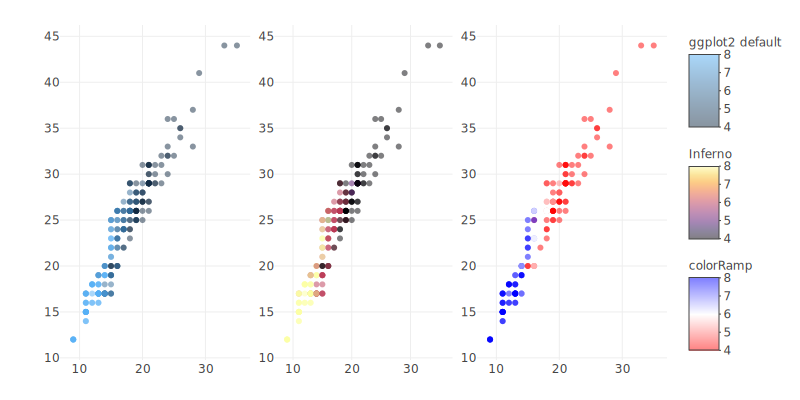
\includegraphics[width=\textwidth]{images/color-numeric} 

}

\caption{(ref:color-numeric)}\label{fig:color-numeric}
\end{figure}

\begin{Shaded}
\begin{Highlighting}[]
\NormalTok{col1 <-}\StringTok{ "Accent"}
\NormalTok{col2 <-}\StringTok{ }\KeywordTok{colorRamp}\NormalTok{(}\KeywordTok{c}\NormalTok{(}\StringTok{"red"}\NormalTok{, }\StringTok{"blue"}\NormalTok{))}
\NormalTok{col3 <-}\StringTok{ }\KeywordTok{c}\NormalTok{(}\StringTok{`}\DataTypeTok{4}\StringTok{`}\NormalTok{ =}\StringTok{ "red"}\NormalTok{, }\StringTok{`}\DataTypeTok{5}\StringTok{`}\NormalTok{ =}\StringTok{ "black"}\NormalTok{, }\StringTok{`}\DataTypeTok{6}\StringTok{`}\NormalTok{ =}\StringTok{ "blue"}\NormalTok{, }\StringTok{`}\DataTypeTok{8}\StringTok{`}\NormalTok{ =}\StringTok{ "green"}\NormalTok{)}
\KeywordTok{subplot}\NormalTok{(}
  \KeywordTok{add_markers}\NormalTok{(p, }\DataTypeTok{color =} \OperatorTok{~}\KeywordTok{factor}\NormalTok{(cyl), }\DataTypeTok{colors =}\NormalTok{ col1),}
  \KeywordTok{add_markers}\NormalTok{(p, }\DataTypeTok{color =} \OperatorTok{~}\KeywordTok{factor}\NormalTok{(cyl), }\DataTypeTok{colors =}\NormalTok{ col2),}
  \KeywordTok{add_markers}\NormalTok{(p, }\DataTypeTok{color =} \OperatorTok{~}\KeywordTok{factor}\NormalTok{(cyl), }\DataTypeTok{colors =}\NormalTok{ col3)}
\NormalTok{) }\OperatorTok\StringTok{ }\KeywordTok{hide_legend}\NormalTok{()}
\end{Highlighting}
\end{Shaded}

\begin{figure}

{\centering 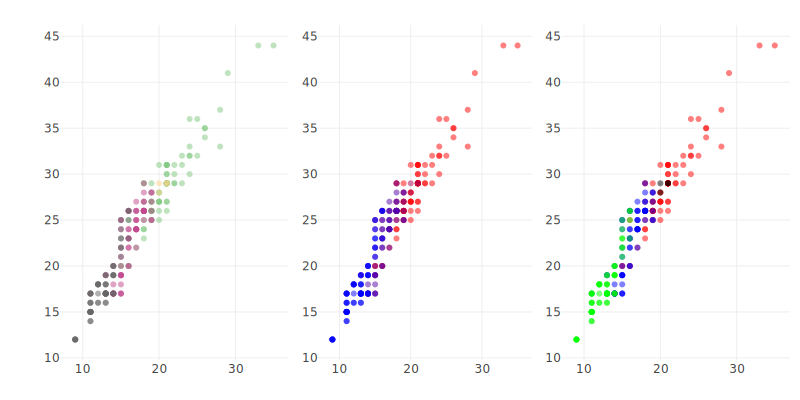
\includegraphics[width=\textwidth]{images/color-discrete} 

}

\caption{(ref:color-discrete)}\label{fig:color-discrete}
\end{figure}

As introduced in Figure \ref{fig:intro-range}, color codes can be specified manually (i.e., avoid mapping data values to a visual range) by using the \texttt{I()} function. Figure \ref{fig:color-manual} provides a simple example using \texttt{add\_markers()}. Any color understood by the \texttt{col2rgb()} function from the \textbf{grDevices} package can be used in this way. Chapter \ref{working-with-colors} provides even more details about working with different color specifications when specifying colors manually.

\begin{Shaded}
\begin{Highlighting}[]
\KeywordTok{add_markers}\NormalTok{(p, }\DataTypeTok{color =} \KeywordTok{I}\NormalTok{(}\StringTok{"black"}\NormalTok{))}
\end{Highlighting}
\end{Shaded}

\begin{figure}

{\centering \includegraphics[width=\textwidth]{images/color-manual} 

}

\caption{(ref:color-manual)}\label{fig:color-manual}
\end{figure}

The \texttt{color} argument is meant to control the `fill-color' of a geometric object, whereas \texttt{stroke} (Section \ref{marker-stroke}) is meant to control the `outline-color' of a geometric object. In the case of \texttt{add\_markers()}, that means \texttt{color} maps to the plotly.js attribute \href{https://plot.ly/r/reference/\#scatter-marker-color}{\texttt{marker.color}} and \texttt{stroke} maps to \href{https://plot.ly/r/reference/\#scatter-marker-line-color}{\texttt{marker.line.color}}. Not all, but many, marker symbols have a notion of stroke.

\hypertarget{marker-symbol}{%
\subsection{Symbols}\label{marker-symbol}}

The \texttt{symbol} argument can be used to map data values to the \texttt{marker.symbol} plotly.js attribute. It uses the same semantics that we've already seen for \texttt{color}:

\begin{itemize}
\tightlist
\item
  A numeric mapping generates trace.
\item
  A discrete mapping generates multiple traces (one trace per category).
\item
  The plural, \texttt{symbols}, can be used to specify the visual range for the mapping.
\item
  Mappings are avoided entirely through \texttt{I()}.
\end{itemize}

For example, the left panel of Figure \ref{fig:symbol-factor} uses a numeric mapping and the right panel uses a discrete mapping. As a result, the left panel is linked to the first legend entry, whereas the right panel is linked to the bottom three legend entries. When plotting multiple traces and no color is specifeid, the plotly.js \href{https://plot.ly/r/reference/\#layout-colorway}{colorway} is applied (i.e., each trace will be rendered a different color). To set a fixed color, you can set the color of every trace generated from this layer with \texttt{color\ =\ I("black")}, or similar.

\begin{Shaded}
\begin{Highlighting}[]
\NormalTok{p <-}\StringTok{ }\KeywordTok{plot_ly}\NormalTok{(mpg, }\DataTypeTok{x =} \OperatorTok{~}\NormalTok{cty, }\DataTypeTok{y =} \OperatorTok{~}\NormalTok{hwy, }\DataTypeTok{alpha =} \FloatTok{0.3}\NormalTok{) }
\KeywordTok{subplot}\NormalTok{(}
  \KeywordTok{add_markers}\NormalTok{(p, }\DataTypeTok{symbol =} \OperatorTok{~}\NormalTok{cyl, }\DataTypeTok{name =} \StringTok{"A single trace"}\NormalTok{),}
  \KeywordTok{add_markers}\NormalTok{(p, }\DataTypeTok{symbol =} \OperatorTok{~}\KeywordTok{factor}\NormalTok{(cyl), }\DataTypeTok{color =} \KeywordTok{I}\NormalTok{(}\StringTok{"black"}\NormalTok{))}
\NormalTok{)}
\end{Highlighting}
\end{Shaded}

\begin{figure}

{\centering \includegraphics[width=\textwidth]{images/symbol-factor} 

}

\caption{(ref:symbol-factor)}\label{fig:symbol-factor}
\end{figure}

There are two ways to specify the visual range of \texttt{symbols}: (1) numeric codes (interpreted as a \texttt{pch} codes) or (2) a character string specifying a valid \texttt{marker.symbol} value. Figure \ref{fig:symbol-factor-range} uses pch codes (left panel) as well as their corresponding \texttt{marker.symbol} name (right panel) to specify the visual range.

\begin{Shaded}
\begin{Highlighting}[]
\KeywordTok{subplot}\NormalTok{(}
  \KeywordTok{add_markers}\NormalTok{(p, }\DataTypeTok{symbol =} \OperatorTok{~}\NormalTok{cyl, }\DataTypeTok{symbols =} \KeywordTok{c}\NormalTok{(}\DecValTok{17}\NormalTok{, }\DecValTok{18}\NormalTok{, }\DecValTok{19}\NormalTok{)),}
  \KeywordTok{add_markers}\NormalTok{(}
\NormalTok{    p, }\DataTypeTok{color =} \KeywordTok{I}\NormalTok{(}\StringTok{"black"}\NormalTok{),}
    \DataTypeTok{symbol =} \OperatorTok{~}\KeywordTok{factor}\NormalTok{(cyl), }
    \DataTypeTok{symbols =} \KeywordTok{c}\NormalTok{(}\StringTok{"triangle-up"}\NormalTok{, }\StringTok{"diamond"}\NormalTok{, }\StringTok{"circle"}\NormalTok{)}
\NormalTok{  )}
\NormalTok{)}
\end{Highlighting}
\end{Shaded}

\begin{figure}

{\centering \includegraphics[width=\textwidth]{images/symbol-factor-range} 

}

\caption{(ref:symbol-factor-range)}\label{fig:symbol-factor-range}
\end{figure}

These \texttt{symbols} (i.e., the visual range) can also be supplied directly to \texttt{symbol} through \texttt{I()}. For example, Figure \ref{fig:symbol-factor-manual} fixes the marker symbol to a diamond shape.

\begin{Shaded}
\begin{Highlighting}[]
\KeywordTok{plot_ly}\NormalTok{(mpg, }\DataTypeTok{x =} \OperatorTok{~}\NormalTok{cty, }\DataTypeTok{y =} \OperatorTok{~}\NormalTok{hwy) }\OperatorTok
\StringTok{  }\KeywordTok{add_markers}\NormalTok{(}\DataTypeTok{symbol =} \KeywordTok{I}\NormalTok{(}\DecValTok{18}\NormalTok{), }\DataTypeTok{alpha =} \FloatTok{0.5}\NormalTok{)}
\end{Highlighting}
\end{Shaded}

\begin{figure}

{\centering 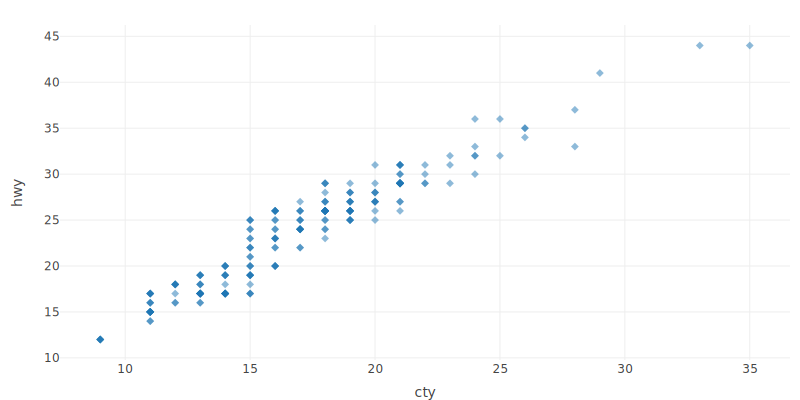
\includegraphics[width=\textwidth]{images/symbol-factor-manual} 

}

\caption{(ref:symbol-factor-manual)}\label{fig:symbol-factor-manual}
\end{figure}

If you'd like to see all the symbols available to \textbf{plotly}, as well as a method for supplying your own custom glyphs, see Chapter \ref{working-with-symbols}.

\hypertarget{marker-stroke}{%
\subsection{Stroke and span}\label{marker-stroke}}

The \texttt{stroke} argument follows the same semantics as \texttt{color} and \texttt{symbol} when it comes to variable mappings and specifying visual ranges. Typically you don't want to map data values to \texttt{stroke}, you just want to specify a fixed outline color. For example, Figure \ref{fig:stroke-manual} modifies Figure \ref{fig:symbol-factor-manual} to simply add a black outline. By default, the \texttt{span}, or width of the stroke, is zero, you'll likely want to set the width to be around one pixel.

\begin{Shaded}
\begin{Highlighting}[]
\KeywordTok{plot_ly}\NormalTok{(mpg, }\DataTypeTok{x =} \OperatorTok{~}\NormalTok{cty, }\DataTypeTok{y =} \OperatorTok{~}\NormalTok{hwy, }\DataTypeTok{alpha =} \FloatTok{0.5}\NormalTok{) }\OperatorTok
\StringTok{  }\KeywordTok{add_markers}\NormalTok{(}\DataTypeTok{symbol =} \KeywordTok{I}\NormalTok{(}\DecValTok{18}\NormalTok{), }\DataTypeTok{stroke =} \KeywordTok{I}\NormalTok{(}\StringTok{"black"}\NormalTok{), }\DataTypeTok{span =} \KeywordTok{I}\NormalTok{(}\DecValTok{1}\NormalTok{))}
\end{Highlighting}
\end{Shaded}

\begin{figure}

{\centering 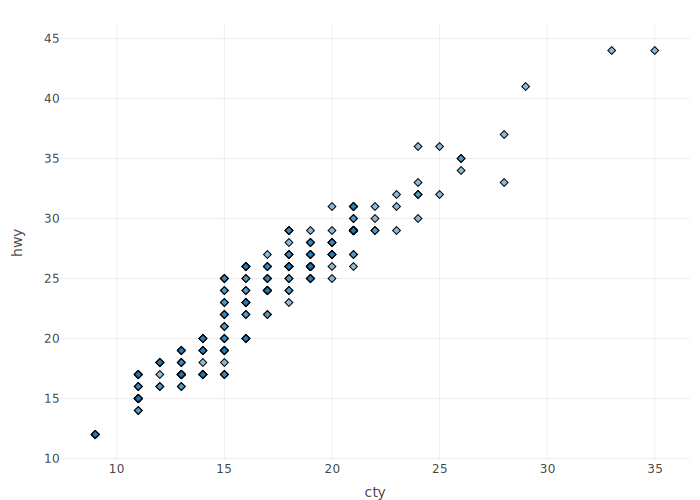
\includegraphics[width=\textwidth]{images/symbol-manual} 

}

\caption{(ref:stroke-manual)}\label{fig:stroke-manual}
\end{figure}

\hypertarget{marker-size}{%
\subsection{Size}\label{marker-size}}

For scatterplots, the \texttt{size} argument controls the area of markers (unless otherwise specified via \href{https://plot.ly/r/reference/\#scatter-marker-sizemode}{sizemode}), and \emph{must} be a numeric variable. The \texttt{sizes} argument controls the minimum and maximum size of circles, in pixels:

\begin{Shaded}
\begin{Highlighting}[]
\NormalTok{p <-}\StringTok{ }\KeywordTok{plot_ly}\NormalTok{(mpg, }\DataTypeTok{x =} \OperatorTok{~}\NormalTok{cty, }\DataTypeTok{y =} \OperatorTok{~}\NormalTok{hwy, }\DataTypeTok{alpha =} \FloatTok{0.3}\NormalTok{) }
\KeywordTok{subplot}\NormalTok{(}
  \KeywordTok{add_markers}\NormalTok{(p, }\DataTypeTok{size =} \OperatorTok{~}\NormalTok{cyl, }\DataTypeTok{name =} \StringTok{"default"}\NormalTok{),}
  \KeywordTok{add_markers}\NormalTok{(p, }\DataTypeTok{size =} \OperatorTok{~}\NormalTok{cyl, }\DataTypeTok{sizes =} \KeywordTok{c}\NormalTok{(}\DecValTok{1}\NormalTok{, }\DecValTok{500}\NormalTok{), }\DataTypeTok{name =} \StringTok{"custom"}\NormalTok{)}
\NormalTok{)}
\end{Highlighting}
\end{Shaded}

\begin{figure}

{\centering 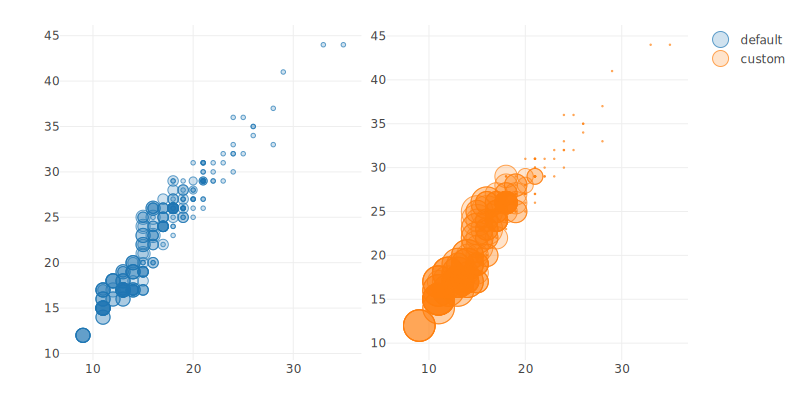
\includegraphics[width=\textwidth]{images/sizes} 

}

\caption{(ref:sizes)}\label{fig:sizes}
\end{figure}

Similar to other arguments, \texttt{I()} can be used to specify the size directly. In the case of markers, \texttt{size} controls the \href{https://plot.ly/r/reference/\#scatter-marker-size}{\texttt{marker.size}} plotly.js attribute. Remember, you always have the option to set this attribute directly by doing something similar to Figure \ref{fig:sizes-manual}.

\begin{Shaded}
\begin{Highlighting}[]
\KeywordTok{plot_ly}\NormalTok{(mpg, }\DataTypeTok{x =} \OperatorTok{~}\NormalTok{cty, }\DataTypeTok{y =} \OperatorTok{~}\NormalTok{hwy, }\DataTypeTok{alpha =} \FloatTok{0.3}\NormalTok{, }\DataTypeTok{size =} \KeywordTok{I}\NormalTok{(}\DecValTok{30}\NormalTok{))}
\end{Highlighting}
\end{Shaded}

\begin{figure}

{\centering 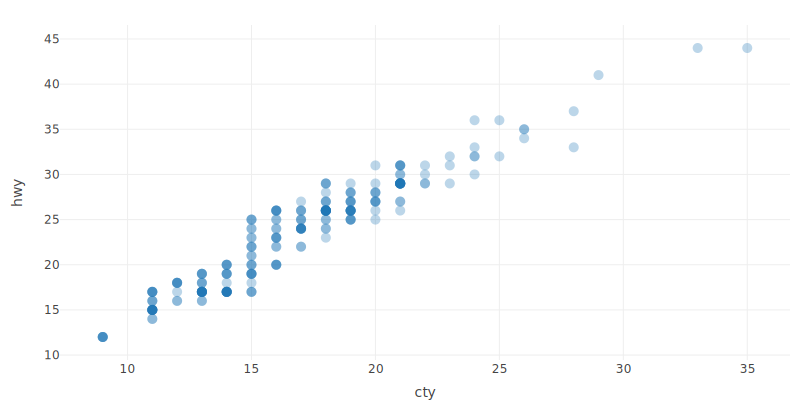
\includegraphics[width=\textwidth]{images/sizes-manual} 

}

\caption{(ref:sizes-manual)}\label{fig:sizes-manual}
\end{figure}

\hypertarget{dot-plots}{%
\subsection{Dotplots \& error bars}\label{dot-plots}}

A dotplot is similar to a scatterplot, except instead of two numeric axes, one is categorical. The usual goal of a dotplot is to compare value(s) on a numerical scale over numerous categories. In this context, dotplots are preferable to pie charts since comparing position along a common scale is much easier than comparing angle or area \citep{graphical-perception, crowdsourcing-graphical-perception}. Furthermore, dotplots can be preferable to bar charts, especially when comparing values within a narrow range far away from 0 \citep{few-values}. Also, when presenting point estimates, and uncertainty associated with those estimates, bar charts tend to exaggerate the difference in point estimates, and lose focus on uncertainty \citep{messing}.

A popular application for dotplots (with error bars) is the so-called ``coefficient plot'' for visualizing the point estimates of coefficients and their standard error. The \texttt{coefplot()} function in the \textbf{coefplot} package \citep{coefplot} and the \texttt{ggcoef()} function in the \textbf{GGally} both produce coefficient plots for many types of model objects in R using \textbf{ggplot2}, which we can translate to plotly via \texttt{ggplotly()}. Since these packages use points and segments to draw the coefficient plots, the hover information is not the best, and it'd be better to use \href{https://plot.ly/r/reference/\#scatter-error_x}{error objects}. Figure \ref{fig:coefplot} uses the \texttt{tidy()} function from the \textbf{broom} package \citep{broom} to obtain a data frame with one row per model coefficient, and produce a coefficient plot with error bars along the x-axis.

\begin{Shaded}
\begin{Highlighting}[]
\CommentTok{# Fit a full-factorial linear model}
\NormalTok{m <-}\StringTok{ }\KeywordTok{lm}\NormalTok{(}
\NormalTok{  Sepal.Length }\OperatorTok{~}\StringTok{ }\NormalTok{Sepal.Width }\OperatorTok{*}\StringTok{ }\NormalTok{Petal.Length }\OperatorTok{*}\StringTok{ }\NormalTok{Petal.Width, }
  \DataTypeTok{data =}\NormalTok{ iris}
\NormalTok{)}

\CommentTok{# (1) get a tidy() data structure of covariate-level info }
\CommentTok{# (e.g., point estimate, standard error, etc)}
\CommentTok{# (2) make sure term column is a factor ordered by the estimate}
\CommentTok{# (3) plot estimate by term with an error bar for the standard error}
\NormalTok{broom}\OperatorTok{::}\KeywordTok{tidy}\NormalTok{(m) }\OperatorTok\StringTok{ }
\StringTok{  }\KeywordTok{mutate}\NormalTok{(}\DataTypeTok{term =}\NormalTok{ forcats}\OperatorTok{::}\KeywordTok{fct_reorder}\NormalTok{(term, estimate)) }\OperatorTok
\StringTok{  }\KeywordTok{plot_ly}\NormalTok{(}\DataTypeTok{x =} \OperatorTok{~}\NormalTok{estimate, }\DataTypeTok{y =} \OperatorTok{~}\NormalTok{term) }\OperatorTok
\StringTok{  }\KeywordTok{add_markers}\NormalTok{(}
    \DataTypeTok{error_x =} \OperatorTok{~}\KeywordTok{list}\NormalTok{(}\DataTypeTok{value =}\NormalTok{ std.error), }
    \DataTypeTok{color =} \KeywordTok{I}\NormalTok{(}\StringTok{"black"}\NormalTok{),}
    \DataTypeTok{hoverinfo =} \StringTok{"x"}
\NormalTok{  )}
\end{Highlighting}
\end{Shaded}

\begin{figure}

{\centering \includegraphics[width=\textwidth]{images/coefplot} 

}

\caption{(ref:coefplot)}\label{fig:coefplot}
\end{figure}

\hypertarget{lines}{%
\section{Lines}\label{lines}}

Many of the same principles we learned about aesthetic mappings with respect to markers (Section \ref{markers}) also apply to lines.\footnote{At the time of writing, the plotly.js attributes \href{https://github.com/plotly/plotly.js/issues/147}{\texttt{line.width} and \texttt{line.color}} do not support multiple values, meaning a single line trace can only have one width/color in 2D line plot, and consequently numeric \texttt{color}/\texttt{size} mappings won't work. This isn't necessarily true for 3D paths/lines and there will likely be support these features for 2D paths/lines in WebGL in the near future.} Moreover, at the start of this chapter (namely Figure \ref{fig:scatter-lines}) we also learned how to use \textbf{dplyr}'s \texttt{group\_by()} to ensure there is at least one geometry (in this case, line) per group. We also learned the difference between \texttt{add\_paths()} and \texttt{add\_lines()} -- the former draws lines according to row ordering whereas the latter draw them according to \texttt{x}. In this chapter, we'll learn about \texttt{linetype}/\texttt{linetype}, an aesthetic that applies to lines and polygons. We'll also discuss some other important chart types that can be implemented with \texttt{add\_paths()}, \texttt{add\_lines()}, and \texttt{add\_segments()}.

\hypertarget{linetypes}{%
\subsection{Linetypes}\label{linetypes}}

Generally speaking, it's hard to perceive more than 8 different colors/linetypes/symbols in a given plot, so sometimes we have to filter data to use these effectively. Here we use the \textbf{dplyr} package to find the top 5 cities in terms of average monthly sales (\texttt{top5}), then effectively filter the original data to contain just these cities via \texttt{semi\_join()}. As Figure \ref{fig:linetypes} demonstrates, once we have the data filtered, mapping city to \texttt{color} or \texttt{linetype} is trivial. The color palette can be altered via the \texttt{colors} argument, and follows the same rules as \protect\hyperlink{scatterplots}{scatterplots}. The linetype palette can be altered via the \texttt{linetypes} argument, and accepts R's \href{https://github.com/wch/r-source/blob/e5b21d0397c607883ff25cca379687b86933d730/src/library/graphics/man/par.Rd\#L726-L743}{\texttt{lty} values} or plotly.js \href{https://plot.ly/r/reference/\#scatter-line-dash}{dash values}.

\begin{Shaded}
\begin{Highlighting}[]
\KeywordTok{library}\NormalTok{(dplyr)}
\NormalTok{top5 <-}\StringTok{ }\NormalTok{txhousing }\OperatorTok
\StringTok{  }\KeywordTok{group_by}\NormalTok{(city) }\OperatorTok
\StringTok{  }\KeywordTok{summarise}\NormalTok{(}\DataTypeTok{m =} \KeywordTok{mean}\NormalTok{(sales, }\DataTypeTok{na.rm =} \OtherTok{TRUE}\NormalTok{)) }\OperatorTok
\StringTok{  }\KeywordTok{arrange}\NormalTok{(}\KeywordTok{desc}\NormalTok{(m)) }\OperatorTok
\StringTok{  }\KeywordTok{top_n}\NormalTok{(}\DecValTok{5}\NormalTok{)}

\NormalTok{tx5 <-}\StringTok{ }\KeywordTok{semi_join}\NormalTok{(txhousing, top5, }\DataTypeTok{by =} \StringTok{"city"}\NormalTok{)}

\KeywordTok{plot_ly}\NormalTok{(tx5, }\DataTypeTok{x =} \OperatorTok{~}\NormalTok{date, }\DataTypeTok{y =} \OperatorTok{~}\NormalTok{median) }\OperatorTok
\StringTok{  }\KeywordTok{add_lines}\NormalTok{(}\DataTypeTok{linetype =} \OperatorTok{~}\NormalTok{city)}
\end{Highlighting}
\end{Shaded}

\begin{figure}

{\centering \includegraphics[width=\textwidth]{images/linetypes} 

}

\caption{(ref:linetypes)}\label{fig:linetypes}
\end{figure}

If you'd like to control exactly which linetype is used to encode a particular data value, you can provide a named character vector, like in Figure \ref{fig:linetypes-manual}. Note that this is similar to how we provided a discrete colorscale manually for markers in Figure \ref{fig:color-discrete}.

\begin{Shaded}
\begin{Highlighting}[]
\NormalTok{ltys <-}\StringTok{ }\KeywordTok{c}\NormalTok{(}
  \DataTypeTok{Austin =} \StringTok{"dashdot"}\NormalTok{,}
  \StringTok{`}\DataTypeTok{Collin County}\StringTok{`}\NormalTok{ =}\StringTok{ "longdash"}\NormalTok{,}
  \DataTypeTok{Dallas =} \StringTok{"dash"}\NormalTok{,}
  \DataTypeTok{Houston =} \StringTok{"solid"}\NormalTok{,}
  \StringTok{`}\DataTypeTok{San Antonio}\StringTok{`}\NormalTok{ =}\StringTok{ "dot"}
\NormalTok{)}

\KeywordTok{plot_ly}\NormalTok{(tx5, }\DataTypeTok{x =} \OperatorTok{~}\NormalTok{date, }\DataTypeTok{y =} \OperatorTok{~}\NormalTok{median) }\OperatorTok
\StringTok{  }\KeywordTok{add_lines}\NormalTok{(}\DataTypeTok{linetype =} \OperatorTok{~}\NormalTok{city, }\DataTypeTok{linetypes =}\NormalTok{ ltys)}
\end{Highlighting}
\end{Shaded}

\begin{figure}

{\centering 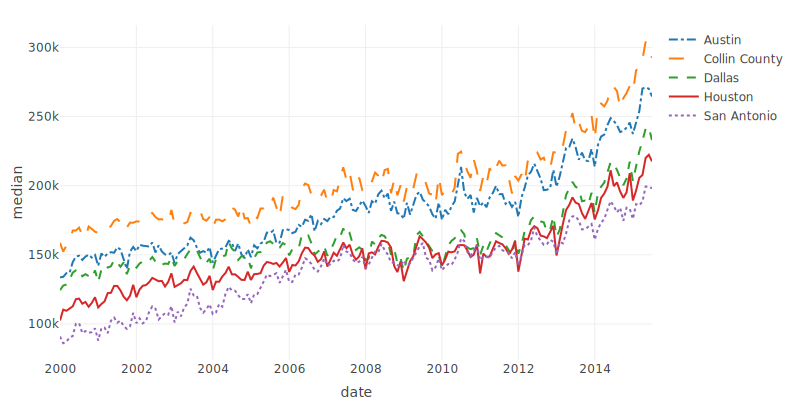
\includegraphics[width=\textwidth]{images/linetypes-manual} 

}

\caption{(ref:linetypes-manual)}\label{fig:linetypes-manual}
\end{figure}

\hypertarget{segments}{%
\subsection{Segments}\label{segments}}

The \texttt{add\_segments()} function essentially provides a way to connect two points {[}(\texttt{x}, \texttt{y}) to (\texttt{xend}, \texttt{yend}){]} with a line. Segments form the building blocks for numerous useful chart types, including slopegraphs, dumbell charts, candlestick charts, and more. Slopegraphs and dumbell charts are useful for comparing numeric values across numerous categories. Candlestick charts are typically used for visualizing change in a financial asset over time.

Segments can also provide a useful alternative to \texttt{add\_bars()} (covered in Chapter \ref{bars-histograms}), especially for animations. In particular, Figure \ref{fig:profile-pyramid} of Section \ref{animation-support} shows how implement an animated population pyramid using segments instead of bars.

\hypertarget{slopegraph}{%
\subsubsection{Slopegraph}\label{slopegraph}}

The slope graph, made popular by \citet{tufte2001}, is a great way to compare the change in a measurement across numerous groups. This change could be along either a discrete or a continuous axis. For a continuous axis, the slopegraph could be thought of as a decomposition of a line graph into multiple segments. The \textbf{slopegraph} R package provides a succinct interface for creating slopegraphs with base or \textbf{ggplot2} graphics and also some convenient data sets which we'll make use of here \citep{slopegraph}. Figure \ref{fig:slopegraph} recreates an example from \citet{tufte2001}, using the \texttt{gdp} data set from \textbf{slopegraph}, and demonstrates a common issue with labelling in slopegraphs -- it's easy to have overlapping labels when anchoring labels on data values. For that reason, this implementation leverages \textbf{plotly} ability to interactively edit annotation positions. See Chapter \ref{editing-views} for similar examples of `editing views'.

\begin{Shaded}
\begin{Highlighting}[]
\KeywordTok{data}\NormalTok{(gdp, }\DataTypeTok{package =} \StringTok{"slopegraph"}\NormalTok{)}
\NormalTok{gdp}\OperatorTok{$}\NormalTok{Country <-}\StringTok{ }\KeywordTok{row.names}\NormalTok{(gdp)}

\KeywordTok{plot_ly}\NormalTok{(gdp) }\OperatorTok
\StringTok{  }\KeywordTok{add_segments}\NormalTok{(}
    \DataTypeTok{x =} \DecValTok{1}\NormalTok{, }\DataTypeTok{xend =} \DecValTok{2}\NormalTok{,}
    \DataTypeTok{y =} \OperatorTok{~}\NormalTok{Year1970, }\DataTypeTok{yend =} \OperatorTok{~}\NormalTok{Year1979,}
    \DataTypeTok{color =} \KeywordTok{I}\NormalTok{(}\StringTok{"gray90"}\NormalTok{)}
\NormalTok{  ) }\OperatorTok
\StringTok{  }\KeywordTok{add_annotations}\NormalTok{(}
    \DataTypeTok{x =} \DecValTok{1}\NormalTok{, }\DataTypeTok{y =} \OperatorTok{~}\NormalTok{Year1970, }
    \DataTypeTok{text =} \OperatorTok{~}\KeywordTok{paste}\NormalTok{(Country, }\StringTok{"  "}\NormalTok{, Year1970), }
    \DataTypeTok{xanchor =} \StringTok{"right"}\NormalTok{, }\DataTypeTok{showarrow =} \OtherTok{FALSE}
\NormalTok{  ) }\OperatorTok
\StringTok{  }\KeywordTok{add_annotations}\NormalTok{(}
    \DataTypeTok{x =} \DecValTok{2}\NormalTok{, }\DataTypeTok{y =} \OperatorTok{~}\NormalTok{Year1979, }
    \DataTypeTok{text =} \OperatorTok{~}\KeywordTok{paste}\NormalTok{(Year1979, }\StringTok{"  "}\NormalTok{, Country),}
    \DataTypeTok{xanchor =} \StringTok{"left"}\NormalTok{, }\DataTypeTok{showarrow =} \OtherTok{FALSE}
\NormalTok{  ) }\OperatorTok
\StringTok{  }\KeywordTok{layout}\NormalTok{(}
    \DataTypeTok{title =} \StringTok{"Current Receipts of Govermnent as a Percentage of GDP"}\NormalTok{,}
    \DataTypeTok{showlegend =} \OtherTok{FALSE}\NormalTok{,}
    \DataTypeTok{xaxis =} \KeywordTok{list}\NormalTok{(}
      \DataTypeTok{range =} \KeywordTok{c}\NormalTok{(}\DecValTok{0}\NormalTok{, }\DecValTok{3}\NormalTok{),}
      \DataTypeTok{ticktext =} \KeywordTok{c}\NormalTok{(}\StringTok{"1970"}\NormalTok{, }\StringTok{"1979"}\NormalTok{),}
      \DataTypeTok{tickvals =} \KeywordTok{c}\NormalTok{(}\DecValTok{1}\NormalTok{, }\DecValTok{2}\NormalTok{),}
      \DataTypeTok{zeroline =} \OtherTok{FALSE}
\NormalTok{    ),}
    \DataTypeTok{yaxis =} \KeywordTok{list}\NormalTok{(}
      \DataTypeTok{title =} \StringTok{""}\NormalTok{,}
      \DataTypeTok{showgrid =} \OtherTok{FALSE}\NormalTok{,}
      \DataTypeTok{showticks =} \OtherTok{FALSE}\NormalTok{,}
      \DataTypeTok{showticklabels =} \OtherTok{FALSE}
\NormalTok{    )}
\NormalTok{  ) }\OperatorTok\StringTok{ }
\StringTok{  }\KeywordTok{config}\NormalTok{(}\DataTypeTok{edits =} \KeywordTok{list}\NormalTok{(}\DataTypeTok{annotationPosition =} \OtherTok{TRUE}\NormalTok{))}
\end{Highlighting}
\end{Shaded}

\begin{figure}

{\centering \includegraphics[width=\textwidth]{vimeo-images/327585190/final} 

}

\caption{(ref:slopegraph)}\label{fig:slopegraph}
\end{figure}

\hypertarget{dumbell}{%
\subsubsection{Dumbell}\label{dumbell}}

So called dumbell charts are similar in concept to slope graphs, but not quite as general. They are typically used to compare two different classes of numeric values across numerous groups. Figure \ref{fig:dumbell} uses the dumbell approach to show average miles per gallon city and highway for different car models. With a dumbell chart, it's always a good idea to order the categories by a sensible metric -- for Figure \ref{fig:dumbell}, the categories are ordered by the city miles per gallon.

\begin{Shaded}
\begin{Highlighting}[]
\NormalTok{mpg }\OperatorTok
\StringTok{  }\KeywordTok{group_by}\NormalTok{(model) }\OperatorTok
\StringTok{  }\KeywordTok{summarise}\NormalTok{(}\DataTypeTok{c =} \KeywordTok{mean}\NormalTok{(cty), }\DataTypeTok{h =} \KeywordTok{mean}\NormalTok{(hwy)) }\OperatorTok
\StringTok{  }\KeywordTok{mutate}\NormalTok{(}\DataTypeTok{model =}\NormalTok{ forcats}\OperatorTok{::}\KeywordTok{fct_reorder}\NormalTok{(model, c)) }\OperatorTok
\StringTok{  }\KeywordTok{plot_ly}\NormalTok{() }\OperatorTok
\StringTok{  }\KeywordTok{add_segments}\NormalTok{(}
    \DataTypeTok{x =} \OperatorTok{~}\NormalTok{c, }\DataTypeTok{y =} \OperatorTok{~}\NormalTok{model,}
    \DataTypeTok{xend =} \OperatorTok{~}\NormalTok{h, }\DataTypeTok{yend =} \OperatorTok{~}\NormalTok{model, }
    \DataTypeTok{color =} \KeywordTok{I}\NormalTok{(}\StringTok{"gray"}\NormalTok{), }\DataTypeTok{showlegend =} \OtherTok{FALSE}
\NormalTok{  ) }\OperatorTok
\StringTok{  }\KeywordTok{add_markers}\NormalTok{(}
    \DataTypeTok{x =} \OperatorTok{~}\NormalTok{c, }\DataTypeTok{y =} \OperatorTok{~}\NormalTok{model, }
    \DataTypeTok{color =} \KeywordTok{I}\NormalTok{(}\StringTok{"blue"}\NormalTok{), }
    \DataTypeTok{name =} \StringTok{"mpg city"}
\NormalTok{  ) }\OperatorTok
\StringTok{  }\KeywordTok{add_markers}\NormalTok{(}
    \DataTypeTok{x =} \OperatorTok{~}\NormalTok{h, }\DataTypeTok{y =} \OperatorTok{~}\NormalTok{model, }
    \DataTypeTok{color =} \KeywordTok{I}\NormalTok{(}\StringTok{"red"}\NormalTok{),}
    \DataTypeTok{name  =} \StringTok{"mpg highway"}
\NormalTok{  ) }\OperatorTok
\StringTok{  }\KeywordTok{layout}\NormalTok{(}\DataTypeTok{xaxis =} \KeywordTok{list}\NormalTok{(}\DataTypeTok{title =} \StringTok{"Miles per gallon"}\NormalTok{))}
\end{Highlighting}
\end{Shaded}

\begin{figure}

{\centering 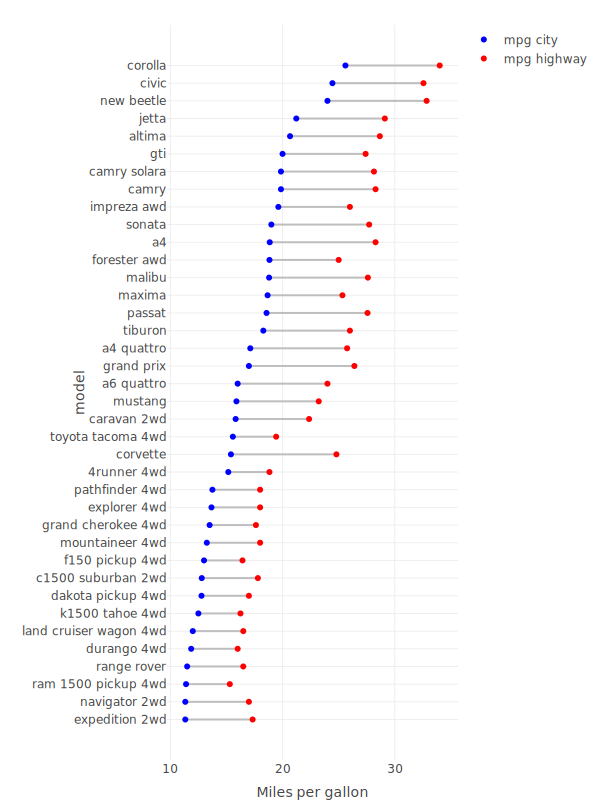
\includegraphics[width=\textwidth]{images/dumbell} 

}

\caption{(ref:dumbell)}\label{fig:dumbell}
\end{figure}

\hypertarget{candlestick}{%
\subsubsection{Candlestick}\label{candlestick}}

Figure \ref{fig:candlestick} uses the \textbf{quantmod} package \citep{quantmod} to obtain stock price data for Microsoft and plots two segments for each day: one to encode the opening/closing values, and one to encode the daily high/low.

\begin{Shaded}
\begin{Highlighting}[]
\KeywordTok{library}\NormalTok{(quantmod)}
\NormalTok{msft <-}\StringTok{ }\KeywordTok{getSymbols}\NormalTok{(}\StringTok{"MSFT"}\NormalTok{, }\DataTypeTok{auto.assign =}\NormalTok{ F)}
\NormalTok{dat <-}\StringTok{ }\KeywordTok{as.data.frame}\NormalTok{(msft)}
\NormalTok{dat}\OperatorTok{$}\NormalTok{date <-}\StringTok{ }\KeywordTok{index}\NormalTok{(msft)}
\NormalTok{dat <-}\StringTok{ }\KeywordTok{subset}\NormalTok{(dat, date }\OperatorTok{>=}\StringTok{ "2016-01-01"}\NormalTok{)}

\KeywordTok{names}\NormalTok{(dat) <-}\StringTok{ }\KeywordTok{sub}\NormalTok{(}\StringTok{"^MSFT}\CharTok{\textbackslash{}\textbackslash{}}\StringTok{."}\NormalTok{, }\StringTok{""}\NormalTok{, }\KeywordTok{names}\NormalTok{(dat))}

\KeywordTok{plot_ly}\NormalTok{(dat, }\DataTypeTok{x =} \OperatorTok{~}\NormalTok{date, }\DataTypeTok{xend =} \OperatorTok{~}\NormalTok{date, }\DataTypeTok{color =} \OperatorTok{~}\NormalTok{Close }\OperatorTok{>}\StringTok{ }\NormalTok{Open, }
        \DataTypeTok{colors =} \KeywordTok{c}\NormalTok{(}\StringTok{"red"}\NormalTok{, }\StringTok{"forestgreen"}\NormalTok{), }\DataTypeTok{hoverinfo =} \StringTok{"none"}\NormalTok{) }\OperatorTok
\StringTok{  }\KeywordTok{add_segments}\NormalTok{(}\DataTypeTok{y =} \OperatorTok{~}\NormalTok{Low, }\DataTypeTok{yend =} \OperatorTok{~}\NormalTok{High, }\DataTypeTok{size =} \KeywordTok{I}\NormalTok{(}\DecValTok{1}\NormalTok{)) }\OperatorTok
\StringTok{  }\KeywordTok{add_segments}\NormalTok{(}\DataTypeTok{y =} \OperatorTok{~}\NormalTok{Open, }\DataTypeTok{yend =} \OperatorTok{~}\NormalTok{Close, }\DataTypeTok{size =} \KeywordTok{I}\NormalTok{(}\DecValTok{3}\NormalTok{)) }\OperatorTok
\StringTok{  }\KeywordTok{layout}\NormalTok{(}\DataTypeTok{showlegend =} \OtherTok{FALSE}\NormalTok{, }\DataTypeTok{yaxis =} \KeywordTok{list}\NormalTok{(}\DataTypeTok{title =} \StringTok{"Price"}\NormalTok{)) }\OperatorTok
\StringTok{  }\KeywordTok{rangeslider}\NormalTok{()}
\end{Highlighting}
\end{Shaded}

\begin{figure}

{\centering 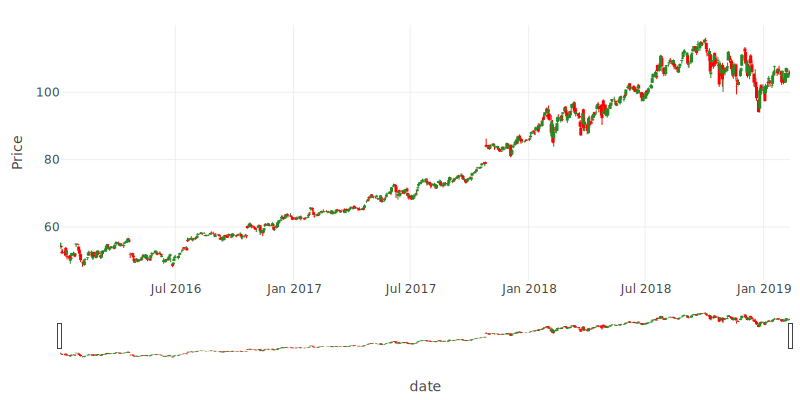
\includegraphics[width=\textwidth]{images/candlestick} 

}

\caption{(ref:candlestick)}\label{fig:candlestick}
\end{figure}

\hypertarget{density-plots}{%
\subsection{Density plots}\label{density-plots}}

In Chapter \ref{bars-histograms}, we leverage a number of algorithms in R for computing the ``optimal'' number of bins for a histogram, via \texttt{hist()}, and routing those results to \texttt{add\_bars()}. We can leverage the \texttt{density()} function for computing kernel density estimates in a similar way, and route the results to \texttt{add\_lines()}, as is done in Figure \ref{fig:densities}.

\begin{Shaded}
\begin{Highlighting}[]
\NormalTok{kerns <-}\StringTok{ }\KeywordTok{c}\NormalTok{(}\StringTok{"gaussian"}\NormalTok{, }\StringTok{"epanechnikov"}\NormalTok{, }\StringTok{"rectangular"}\NormalTok{, }
          \StringTok{"triangular"}\NormalTok{, }\StringTok{"biweight"}\NormalTok{, }\StringTok{"cosine"}\NormalTok{, }\StringTok{"optcosine"}\NormalTok{)}
\NormalTok{p <-}\StringTok{ }\KeywordTok{plot_ly}\NormalTok{()}
\ControlFlowTok{for}\NormalTok{ (k }\ControlFlowTok{in}\NormalTok{ kerns) \{}
\NormalTok{  d <-}\StringTok{ }\KeywordTok{density}\NormalTok{(economics}\OperatorTok{$}\NormalTok{pce, }\DataTypeTok{kernel =}\NormalTok{ k, }\DataTypeTok{na.rm =} \OtherTok{TRUE}\NormalTok{)}
\NormalTok{  p <-}\StringTok{ }\KeywordTok{add_lines}\NormalTok{(p, }\DataTypeTok{x =}\NormalTok{ d}\OperatorTok{$}\NormalTok{x, }\DataTypeTok{y =}\NormalTok{ d}\OperatorTok{$}\NormalTok{y, }\DataTypeTok{name =}\NormalTok{ k)}
\NormalTok{\}}
\NormalTok{p}
\end{Highlighting}
\end{Shaded}

\begin{figure}

{\centering 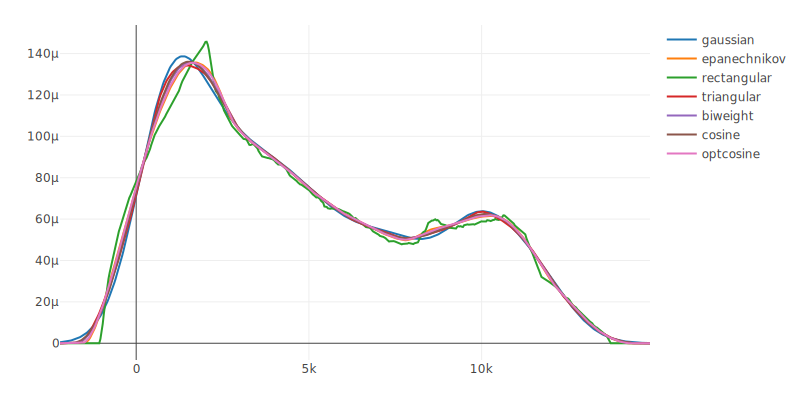
\includegraphics[width=\textwidth]{images/densities} 

}

\caption{(ref:densities)}\label{fig:densities}
\end{figure}

\hypertarget{parallel-coordinates}{%
\subsection{Parallel Coordinates}\label{parallel-coordinates}}

One very useful, but often overlooked, visualization technique is the parallel coordinates plot. Parallel coordinates provide a way to compare values along a common (or non-aligned) positional scale(s) -- the most basic of all perceptual tasks -- in more than 3 dimensions \citep{graphical-perception}. Usually each line represents every measurement for a given row (or observation) in a data set. It's true that plotly.js provides a trace type, parcoords, specifically for parallel coordinates that offers desirable interactive capabilities (e.g., highlighting and reordering of axes).\footnote{See \url{https://plot.ly/r/parallel-coordinates-plot/} for some interactive examples}. However, it can also be useful learn how to use \texttt{add\_lines()} to implement parallel coordinates as it can offer more flexibility and control over the axis scales.

When measurements are on very different scales, some care must be taken, and variables must transformed to be put on a common scale. As Figure \ref{fig:pcp-common} shows, even when variables are measured on a similar scale, it can still be informative to transform variables in different ways.

\begin{Shaded}
\begin{Highlighting}[]
\NormalTok{iris}\OperatorTok{$}\NormalTok{obs <-}\StringTok{ }\KeywordTok{seq_len}\NormalTok{(}\KeywordTok{nrow}\NormalTok{(iris))}
\NormalTok{iris_pcp <-}\StringTok{ }\ControlFlowTok{function}\NormalTok{(}\DataTypeTok{transform =}\NormalTok{ identity) \{}
\NormalTok{  iris[] <-}\StringTok{ }\NormalTok{purrr}\OperatorTok{::}\KeywordTok{map_if}\NormalTok{(iris, is.numeric, transform)}
\NormalTok{  tidyr}\OperatorTok{::}\KeywordTok{gather}\NormalTok{(iris, variable, value, }\OperatorTok{-}\NormalTok{Species, }\OperatorTok{-}\NormalTok{obs) }\OperatorTok\StringTok{ }
\StringTok{    }\KeywordTok{group_by}\NormalTok{(obs) }\OperatorTok\StringTok{ }
\StringTok{    }\KeywordTok{plot_ly}\NormalTok{(}\DataTypeTok{x =} \OperatorTok{~}\NormalTok{variable, }\DataTypeTok{y =} \OperatorTok{~}\NormalTok{value, }\DataTypeTok{color =} \OperatorTok{~}\NormalTok{Species) }\OperatorTok\StringTok{ }
\StringTok{    }\KeywordTok{add_lines}\NormalTok{(}\DataTypeTok{alpha =} \FloatTok{0.3}\NormalTok{)}
\NormalTok{\}}
\KeywordTok{subplot}\NormalTok{(}
  \KeywordTok{iris_pcp}\NormalTok{(), }
  \KeywordTok{iris_pcp}\NormalTok{(scale),}
  \KeywordTok{iris_pcp}\NormalTok{(scales}\OperatorTok{::}\NormalTok{rescale),}
  \DataTypeTok{nrows =} \DecValTok{3}\NormalTok{, }\DataTypeTok{shareX =} \OtherTok{TRUE}
\NormalTok{) }\OperatorTok\StringTok{ }\KeywordTok{hide_legend}\NormalTok{()}
\end{Highlighting}
\end{Shaded}

\begin{figure}

{\centering 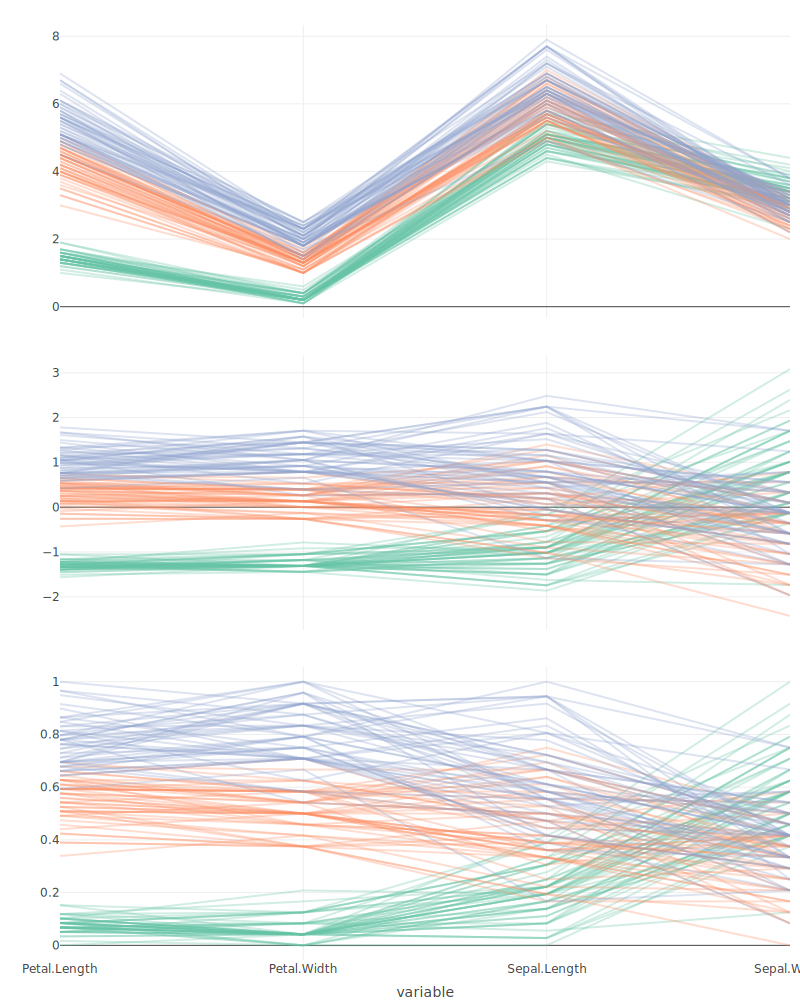
\includegraphics[width=\textwidth]{images/pcp-common} 

}

\caption{(ref:pcp-common)}\label{fig:pcp-common}
\end{figure}

It is also worth noting that the \textbf{GGally} offers a \texttt{ggparcoord()} function which creates parallel coordinate plots via \textbf{ggplot2}, which we can convert to plotly via \texttt{ggplotly()}. Thanks to the \protect\hyperlink{linking-views-without-shiny}{linked highlighting} framework, parallel coordinates created in this way could be linked to lower dimensional (but sometimes higher resolution) graphics of related data to guide multi-variate data exploration. The \textbf{pedestrians} package provides some examples of linking parallel coordinates to other views such as a grand tour for exposing unusual features in a high-dimensional space \citep{pedestrians}.

\hypertarget{polygons}{%
\section{Polygons}\label{polygons}}

The \texttt{add\_polygons()} function is essentially equivalent to \texttt{add\_paths()} with the \href{https://plot.ly/r/reference/\#scatter-fill}{fill} attribute set to ``toself''. Polygons form the basis for other, higher-level scatter-based layers (e.g., \texttt{add\_ribbons()} and \texttt{add\_sf()}) that don't have a dedicated plotly.js trace type. Polygons can be use to draw many things, but perhaps the most familiar application where you \emph{might} want to use \texttt{add\_polygons()} is to draw geo-spatial objects. If and when you use \texttt{add\_polygons()} to draw a map, make sure you fix the aspect ratio (e.g., \href{https://plot.ly/r/reference/\#layout-xaxis-scaleanchor}{\texttt{xaxis.scaleanchor}}) and also consider using \texttt{plotly\_empty()} over \texttt{plot\_ly()} to hide axis labels, ticks, and the background grid. On the other hand, Section \ref{maps-custom} shows you how to make a custom maps using the \textbf{sf} package and \texttt{add\_sf()}, which is a bit of work to get started, but is absolutely worth the investment.

\begin{Shaded}
\begin{Highlighting}[]
\NormalTok{base <-}\StringTok{ }\KeywordTok{map_data}\NormalTok{(}\StringTok{"world"}\NormalTok{, }\StringTok{"canada"}\NormalTok{) }\OperatorTok
\StringTok{  }\KeywordTok{group_by}\NormalTok{(group) }\OperatorTok
\StringTok{  }\KeywordTok{plotly_empty}\NormalTok{(}\DataTypeTok{x =} \OperatorTok{~}\NormalTok{long, }\DataTypeTok{y =} \OperatorTok{~}\NormalTok{lat, }\DataTypeTok{alpha =} \FloatTok{0.2}\NormalTok{) }\OperatorTok
\StringTok{  }\KeywordTok{layout}\NormalTok{(}\DataTypeTok{showlegend =} \OtherTok{FALSE}\NormalTok{, }\DataTypeTok{xaxis =} \KeywordTok{list}\NormalTok{(}\DataTypeTok{scaleanchor =} \StringTok{"y"}\NormalTok{))}
  
\NormalTok{base }\OperatorTok
\StringTok{  }\KeywordTok{add_polygons}\NormalTok{(}\DataTypeTok{hoverinfo =} \StringTok{"none"}\NormalTok{, }\DataTypeTok{color =} \KeywordTok{I}\NormalTok{(}\StringTok{"black"}\NormalTok{)) }\OperatorTok
\StringTok{  }\KeywordTok{add_markers}\NormalTok{(}\DataTypeTok{text =} \OperatorTok{~}\KeywordTok{paste}\NormalTok{(name, }\StringTok{"<br />"}\NormalTok{, pop), }\DataTypeTok{hoverinfo =} \StringTok{"text"}\NormalTok{, }
              \DataTypeTok{color =} \KeywordTok{I}\NormalTok{(}\StringTok{"red"}\NormalTok{), }\DataTypeTok{data =}\NormalTok{ maps}\OperatorTok{::}\NormalTok{canada.cities)}
\end{Highlighting}
\end{Shaded}

\begin{figure}

{\centering 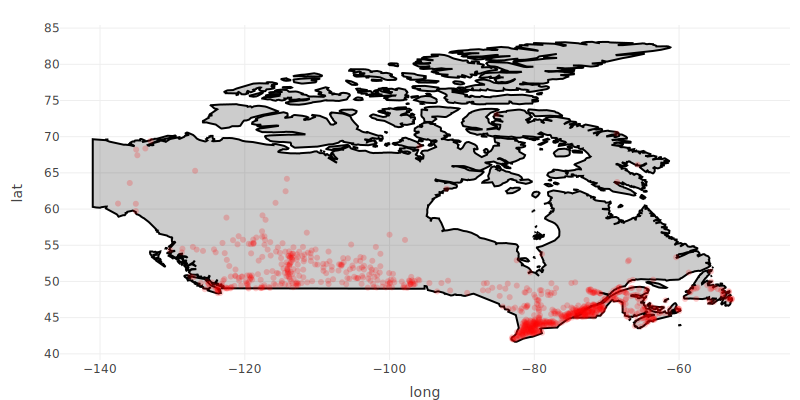
\includegraphics[width=\textwidth]{images/map-canada} 

}

\caption{(ref:map-canada)}\label{fig:map-canada}
\end{figure}

As discussion surrounding Figure \ref{fig:split-color} points out, scatter-based polygon layers (i.e., \texttt{add\_polygons()}, \texttt{add\_ribbons()}, etc) render all the polygons using one plotly.js trace by default. This approach is computationally efficient, but it's not always desirable (e.g., can't have multiple fills per trace, interactivity is relatively limited). To work around the limitations, consider using \texttt{split} (or \texttt{color} with a discrete variable) to split the polygon data into multiple traces. Figure \ref{fig:map-canada-split} demonstrates using \texttt{split} which will impose plotly.js' colorway to each trace (i.e., subregion) and leverage \texttt{hoveron} to generate one tooltip per sub-region.

\begin{Shaded}
\begin{Highlighting}[]
\KeywordTok{add_polygons}\NormalTok{(base, }\DataTypeTok{split =} \OperatorTok{~}\NormalTok{subregion, }\DataTypeTok{hoveron =} \StringTok{"fills"}\NormalTok{)}
\end{Highlighting}
\end{Shaded}

\begin{figure}

{\centering \includegraphics[width=\textwidth]{images/map-canada-split} 

}

\caption{(ref:map-canada-split)}\label{fig:map-canada-split}
\end{figure}

\hypertarget{ribbons}{%
\subsection{Ribbons}\label{ribbons}}

Ribbons are useful for showing uncertainty bounds as a function of x. The \texttt{add\_ribbons()} function creates ribbons and requires the arguments: \texttt{x}, \texttt{ymin}, and \texttt{ymax}. The \texttt{augment()} function from the \textbf{broom} package appends observational-level model components (e.g., fitted values stored as a new column \texttt{.fitted}) which is useful for extracting those components in a convenient form for visualization. Figure \ref{fig:broom-lm} shows the fitted values and uncertainty bounds from a linear model object.

\begin{Shaded}
\begin{Highlighting}[]
\NormalTok{m <-}\StringTok{ }\KeywordTok{lm}\NormalTok{(mpg }\OperatorTok{~}\StringTok{ }\NormalTok{wt, }\DataTypeTok{data =}\NormalTok{ mtcars)}
\NormalTok{broom}\OperatorTok{::}\KeywordTok{augment}\NormalTok{(m) }\OperatorTok
\StringTok{  }\KeywordTok{plot_ly}\NormalTok{(}\DataTypeTok{x =} \OperatorTok{~}\NormalTok{wt, }\DataTypeTok{showlegend =} \OtherTok{FALSE}\NormalTok{) }\OperatorTok
\StringTok{  }\KeywordTok{add_markers}\NormalTok{(}\DataTypeTok{y =} \OperatorTok{~}\NormalTok{mpg, }\DataTypeTok{color =} \KeywordTok{I}\NormalTok{(}\StringTok{"black"}\NormalTok{)) }\OperatorTok
\StringTok{  }\KeywordTok{add_ribbons}\NormalTok{(}\DataTypeTok{ymin =} \OperatorTok{~}\NormalTok{.fitted }\OperatorTok{-}\StringTok{ }\FloatTok{1.96} \OperatorTok{*}\StringTok{ }\NormalTok{.se.fit, }
              \DataTypeTok{ymax =} \OperatorTok{~}\NormalTok{.fitted }\OperatorTok{+}\StringTok{ }\FloatTok{1.96} \OperatorTok{*}\StringTok{ }\NormalTok{.se.fit, }
              \DataTypeTok{color =} \KeywordTok{I}\NormalTok{(}\StringTok{"gray80"}\NormalTok{)) }\OperatorTok
\StringTok{  }\KeywordTok{add_lines}\NormalTok{(}\DataTypeTok{y =} \OperatorTok{~}\NormalTok{.fitted, }\DataTypeTok{color =} \KeywordTok{I}\NormalTok{(}\StringTok{"steelblue"}\NormalTok{))}
\end{Highlighting}
\end{Shaded}

\begin{figure}

{\centering 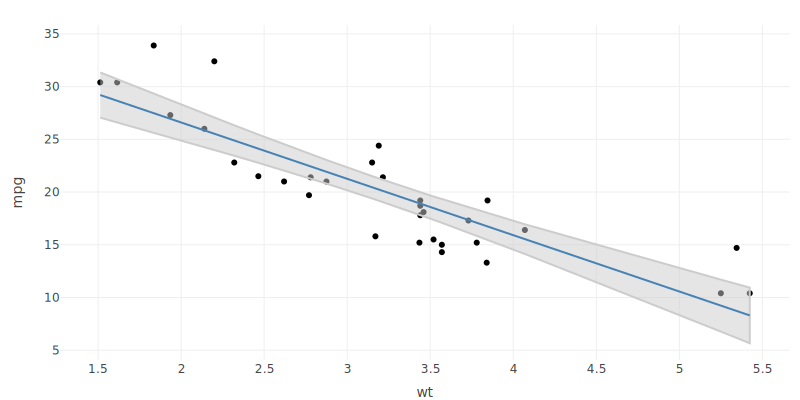
\includegraphics[width=\textwidth]{images/broom-lm} 

}

\caption{(ref:broom-lm)}\label{fig:broom-lm}
\end{figure}

  \bibliography{book.bib,packages.bib}

\backmatter
\printindex

\end{document}
